\documentclass[11pt,a4paper]{article}

% ── Packages ──────────────────────────────────────────────
\usepackage[utf8]{inputenc}
\usepackage[T1]{fontenc}
\usepackage{amsmath,amssymb}
\usepackage{graphicx}
\usepackage{booktabs}
\usepackage[round]{natbib}
\usepackage{hyperref}
\usepackage[margin=2.5cm]{geometry}

% ── Title ─────────────────────────────────────────────────
\title{Affective Valence and Temporal Framing:\\
       A Computational Theory of Counterfactual Precision Redistribution}
\author{Mahault Albarracin}
\date{}

\begin{document}
\maketitle

\begin{abstract}
Emotions are temporally structured: regret concerns what has happened, anxiety concerns what will happen, and surprise concerns what is happening now. Within predictive processing, variational free energy (VFE) evaluates how well the agent's model fits past observations, while expected free energy (EFE) evaluates how well future observations will match preferences. We propose that this computational distinction provides a unified temporal taxonomy of affect: emotions inherit their temporal direction from whichever free energy quantity generates them. Building on this mapping, we formalise counterfactual temporal framing as the mechanism by which agents actively navigate the temporal structure of affect. Temporal framing is cast as policy selection within a partially observable Markov decision process, where each policy redistributes precision across temporal horizons via distinct transition matrices. We show that this redistribution emerges naturally from EFE minimisation: high prediction error favours future-oriented framing (prospective counterfactual simulation), while stable beliefs with high positive-belief precision favour past-oriented framing (autobiographical narrative stabilisation). A three-channel valence decomposition, separating backward (model valence), present (reward valence), and forward (action valence) components, provides a direct readout of temporal orientation at each timestep. Simulations demonstrate that healthy agents balance temporal orientations adaptively, with past-oriented framing serving as a preparatory step for present engagement. Two extensions to the standard active inference framework capture key features of affective pathology: \emph{asymmetric hedonic sensitivity}, where separate precision parameters for positive and negative outcomes model the reward-processing asymmetry observed in depression, and \emph{habit priors} (E~vectors), where additive log-priors over policies model the habitual, EFE-suboptimal action tendencies characteristic of rumination. Chronic stress produces a pathological pattern: elevated future frame beliefs with depleted present engagement, persistent negative reward valence from frustrated forward projection, and a self-amplifying cycle where precise future predictions are systematically violated by a volatile environment. Depression emerges as past-directed ruminative fixation: a strong habit prior toward RECALL, combined with asymmetric punishment sensitivity ($c_{\text{neg}} \gg c_{\text{pos}}$), locks the agent into past-oriented framing with persistently negative reward valence despite near-zero composite affect (anhedonia). We connect this framework to the mood--emotion timescale hierarchy, validate it against ten emotion profiles in the Pleasure--Arousal--Dominance space, and situate it within the broader project of temporal aiming in active inference.
\end{abstract}


\section{Introduction}\label{sec:introduction}

How do organisms decide where in time to direct their attention? A key insight of predictive processing is that affect is not a post-hoc label attached to perception but an integral part of the inference process itself \citep{barrett2017theory, seth2016interoceptive}. Valence, on this account, reflects the rate of change of the agent's model fit to its environment \citep{joffily2013emotional}: improving fit produces positive valence, deteriorating fit produces negative valence. This formulation grounds affect in the same variational free energy (VFE) quantity that drives perception and learning.

A complementary strand of work has shown that affect is also forward-looking. Expected free energy (EFE), the quantity minimised in active inference policy selection \citep{parr2022active}, evaluates how well future observations will match preferences under each available policy. \citet{hesp2021deeply} showed that the ``affective charge'' of policy revision, that is, the degree to which the agent shifts probability toward better policies, constitutes a forward-looking valence signal. \citet{pattisapu2024free} extended the affective readout to include a present-oriented reward prediction error channel, completing a three-channel architecture spanning backward, present, and forward temporal orientations.

These contributions establish that affect has temporal structure. Yet no existing paper formally unifies the VFE/EFE distinction into a temporal taxonomy of emotion, nor provides a computational model of how organisms \emph{actively navigate} this temporal structure. \citet{hinrichs2025temporal} introduced ``temporal aiming'' in the context of geometric hyperscanning, showing how coupled active inference agents coordinate their affective temporal orientations during dyadic interaction. However, the single-agent computational mechanism, the process by which an individual agent selects which temporal horizon of free energy dominates its affective signal, remains unaddressed.

This paper fills both gaps. We formally propose the VFE/EFE temporal mapping as a unified theory of affective temporal direction (\S\ref{sec:temporal_structure}), derive a three-channel valence architecture that decomposes affect into its temporal components (\S\ref{sec:three_channel}), and formalise counterfactual temporal framing as precision redistribution across temporal horizons (\S\ref{sec:counterfactual}). Temporal framing is not a separate cognitive function bolted onto inference; it \emph{emerges} from EFE minimisation given the right generative model structure. We introduce two extensions to the standard active inference apparatus: \emph{asymmetric hedonic sensitivity} ($c_{\text{pos}} \neq c_{\text{neg}}$), which captures the reward-processing asymmetry observed in depression \citep{eshel2010reward, pizzagalli2014depression}, and \emph{habit priors} (E~vectors, following \citealt{dacosta2020active}), which model the habitual, EFE-suboptimal tendencies characteristic of depressive rumination \citep{nolenhoeksema1991responses}. We demonstrate the framework with simulations of past-oriented framing (\S\ref{sec:past}), future-oriented framing (\S\ref{sec:future}), the pathological case of chronic stress as maladaptive temporal fixation (\S\ref{sec:chronic_stress}), and validate it against ten emotion profiles spanning the PAD space (\S\ref{sec:pad_validation}).

The generative model is sufficiently general to accommodate clinical applications, such as bipolar disorder modelling, though here we focus on the temporal mechanism itself.


\section{The Temporal Structure of Free Energy}\label{sec:temporal_structure}

\subsection{VFE as Backward-Looking Evaluation}\label{sec:vfe}

Variational free energy provides the fundamental backward-looking evaluation in active inference. For a generative model $p(o, s)$ with approximate posterior $q(s)$ over hidden states $s$ given observations $o$:
\begin{equation}
    F = \underbrace{-\mathbb{E}_{q(s)}[\ln p(o \mid s)]}_{\text{accuracy}} + \underbrace{D_{\mathrm{KL}}[q(s) \,\|\, p(s)]}_{\text{complexity}}
\end{equation}
$F$ evaluates how well the \emph{current} model fits \emph{past} observations: accuracy measures the expected log-likelihood of what has already been observed, while complexity penalises deviation from prior beliefs. Minimising $F$ with respect to $q(s)$ is perception; minimising $F$ with respect to $p(o,s)$ is learning.

\citet{joffily2013emotional} showed that the temporal derivative of $F$ provides a natural valence signal:
\begin{equation}
    -\frac{dF}{dt}: \quad \text{rate of model improvement}
\end{equation}
Decreasing $F$ (improving model fit) produces positive valence; increasing $F$ produces negative valence. This is inherently backward-looking: it evaluates the \emph{trajectory} of model fit over recent observations.

The second temporal derivative $-d^2F/dt^2$ further differentiates affective states by their dynamics. When both $dF$ and $d^2F$ are negative, the model fit is improving at an accelerating rate, corresponding to \textbf{hope}. When $dF$ is negative but $d^2F$ is positive, improvement is decelerating and stabilising into a good state, corresponding to \textbf{happiness}. Conversely, when both are positive, model fit is worsening at an accelerating rate, corresponding to \textbf{fear}, while negative $d^2F$ with positive $dF$ indicates stabilisation into a bad state, corresponding to \textbf{unhappiness}. Sign changes in $dF$ mark affective transitions: a shift from positive to negative $dF$ corresponds to \textbf{relief}, while a shift from negative to positive corresponds to \textbf{disappointment}. This taxonomy derives entirely from the dynamics of a single backward-looking quantity.

\subsection{EFE as Forward-Looking Evaluation}\label{sec:efe}

Expected free energy provides the complementary forward-looking evaluation. For a policy $\pi$ that produces predicted future observations:
\begin{equation}
    G(\pi) = \sum_m \left[\underbrace{D_{\mathrm{KL}}[q(o_m \mid \pi) \,\|\, p(o_m \mid C_m)]}_{\text{risk}_m} + \underbrace{\mathbb{E}_{q(s)}[H[p(o_m \mid s)]]}_{\text{ambiguity}_m}\right]
\end{equation}
where the sum ranges over observation modalities $m$, $q(o_m \mid \pi)$ is the predicted observation distribution under policy $\pi$, and $p(o_m \mid C_m)$ encodes preferences. Risk measures the divergence between predicted and preferred observations; ambiguity measures the expected entropy of the observation model.

$G(\pi)$ evaluates how well \emph{future} observations will match preferences: it asks not ``did I predict well?'' (VFE) but ``will I predict well?'' (EFE). This temporal complement is the foundation of the mapping we propose.

\subsection{The VFE/EFE Temporal Mapping}\label{sec:temporal_mapping}

We propose that emotions inherit their temporal direction from whichever free energy quantity generates them. This yields a systematic taxonomy.

\paragraph{Backward (VFE-generated).} Emotions grounded in the evaluation of past model fit include \emph{regret} (VFE higher than counterfactual alternative), \emph{guilt} (VFE elevated due to own action), \emph{shame} (VFE elevated due to social model violation), \emph{pride} (VFE lower than expected), and \emph{gratitude} (VFE reduction attributed to another agent).

\paragraph{Present ($-dF/dt$ or RPE).} Emotions grounded in the rate of change at the current moment include \emph{joy} (rapid VFE decrease), \emph{anger} (VFE increase attributed to external agent), \emph{disgust} (VFE increase in interoceptive modality), and \emph{surprise} (large absolute $\Delta F$).

\paragraph{Forward (EFE-generated).} Emotions grounded in the evaluation of expected future performance include \emph{hope} (low EFE under preferred policy), \emph{fear} (high EFE across all policies), \emph{anxiety} (high EFE with high ambiguity), and \emph{anticipation} (low EFE with low ambiguity).

\paragraph{Transitional (VFE vs prior EFE).} Emotions that arise from comparing current VFE with previously computed EFE include \emph{relief} (VFE lower than EFE had predicted), \emph{disappointment} (VFE higher than EFE had predicted), and \emph{satisfaction} (VFE confirms low EFE prediction).

This mapping extends the appraisal-theoretic classification of \citet{smith1985patterns} and the OCC model of \citet{ortony1988cognitive} by grounding the temporal dimension in the formal distinction between variational and expected free energy, rather than in folk-psychological temporal labels.

\subsection{Counterfactual Emotions and Temporal Simulation}\label{sec:counterfactual_emotions}

A particularly revealing class of emotions requires maintaining beliefs about unchosen policies. \citet{hesp2020sophisticated} showed that \emph{sophisticated} affective inference involves evaluating counterfactual trajectories: the agent computes what \emph{would have} happened under alternative policies, and the divergence between actual and counterfactual VFE generates emotions like regret and relief.

Formally, regret at time $t$ is:
\begin{equation}
    \text{Regret} = F_{\text{actual}}(t) - \min_{\pi'} F_{\text{counterfactual}}(t \mid \pi')
\end{equation}
Computing $F_{\text{counterfactual}}$ requires running the generative model \emph{offline}, simulating what would have happened under the unchosen policy. This is exactly what temporal framing does: the agent simulates past states (RECALL) or future states (FUTURATE) by running its generative model in a mode decoupled from current sensory input. Counterfactual emotions thus require the same computational machinery as temporal framing, suggesting that temporal framing may be the general mechanism and counterfactual emotions its specific affective products.


\section{Three-Channel Valence as Temporal Derivative Decomposition}\label{sec:three_channel}

\subsection{Three Readings from the Inference Pipeline}\label{sec:pipeline}

Each valence channel reads from a different point in the agent's processing loop:
\begin{equation}
    \text{observation} \to \underbrace{\text{belief update}}_{\to\, v_{\text{model}}} \to \underbrace{\text{EFE recomputation}}_{\to\, v_{\text{reward}}} \to \underbrace{\text{policy update}}_{\to\, v_{\text{action}}}
\end{equation}
This sequential structure means the three channels are not independent measurements of the same quantity but successive evaluations at increasing temporal remove from the current observation.

\subsection{Channel 1: Model Valence $v_{\text{model}}$ (Backward)}\label{sec:v_model}

Following \citet{joffily2013emotional}, model valence tracks the rate of change of variational free energy:
\begin{equation}
    v_{\text{model}} = \tanh\!\left(\frac{-\Delta F}{\tau_{\text{model}}}\right)
\end{equation}
where $\Delta F = F(t) - F(t{-}1)$. Decreasing free energy (improving model fit) produces positive valence; increasing free energy produces negative valence.

This channel has a natural functional role: it modulates the \emph{model} learning rate (distinct from the arousal-driven \emph{policy} precision discussed in \S\ref{sec:loop}). Persistently negative $v_{\text{model}}$ signals that the generative model is deteriorating, which should accelerate parameter updating ($\sigma_{\text{eff}} = \sigma \times \exp(-\alpha \cdot v_{\text{model}})$). Its temporal character is strictly backward: it evaluates the current state relative to the model's past predictions.

\subsection{Channel 2: Reward Valence $v_{\text{reward}}$ (Present)}\label{sec:v_reward}

Following \citet{pattisapu2024free}, reward valence captures the momentary reward prediction error:
\begin{equation}
    v_{\text{reward}} = \tanh\!\left(\frac{U - \mathbb{E}[U]}{\tau_{\text{reward}}}\right)
\end{equation}
where $U = \sum_{m \in \mathcal{H}} \log P(o_m \mid C_m)$ is the utility of the observed outcome and $\mathbb{E}[U] = \sum_{m \in \mathcal{H}} \sum_o Q(o_m) \log P(o_m \mid C_m)$ is the expected utility under predicted observations, restricted to the \emph{hedonic} modalities $\mathcal{H} = \{o_{\text{ext}}, o_{\text{val}}\}$. The interoceptive modality is excluded from felt valence because body-budget maintenance is largely preconscious \citep{seth2016interoceptive, barrett2017theory}: interoceptive prediction errors drive allostatic regulation (via the EFE policy selection) but do not produce conscious hedonic experience.

This channel drives preference monitoring: chronic negative $v_{\text{reward}}$ signals that the agent's preferences ($\mathbf{C}$ vectors) may be unrealistic. Its temporal character is present-oriented: it evaluates \emph{this} observation relative to what was expected.

\subsection{Channel 3: Action Valence $v_{\text{action}}$ (Forward)}\label{sec:v_action}

Following \citet{hesp2021deeply}, action valence captures the affective charge of policy revision:
\begin{equation}
    v_{\text{action}} = \tanh\!\left(\frac{\text{AC}}{\tau_{\text{action}}}\right), \qquad \text{AC} = (\boldsymbol{\pi}_{t-1} - \boldsymbol{\pi}_t) \cdot \mathbf{G}
\end{equation}
where $\boldsymbol{\pi}$ is the policy distribution and $\mathbf{G}$ the expected free energy vector. Positive affective charge indicates the agent is shifting probability \emph{away from} high-EFE policies (planning improvement); negative charge indicates deterioration.

This channel drives precision updating: positive $v_{\text{action}}$ increases the effective inverse temperature $\bar{\beta}$ (more decisive policy selection), while negative $v_{\text{action}}$ decreases it (more exploratory). Its temporal character is forward-looking: it evaluates whether the agent's \emph{planning} is improving.

\subsection{Composite Valence and Channel Disagreement}\label{sec:composite}

The three channels combine into a single bounded signal:
\begin{equation}
    V = \tanh(v_{\text{model}} + v_{\text{reward}} + v_{\text{action}})
\end{equation}

When channels agree, the affective signal is unambiguous: genuine satisfaction when all are positive, or genuine distress when all are negative. When they disagree, the resulting states are informationally rich. A state of \emph{productive failure} arises when $v_{\text{model}} < 0$ and $v_{\text{action}} > 0$: the current observation was bad, but the agent found a better plan, corresponding to learning from mistakes. \emph{Unsettling success} occurs when $v_{\text{reward}} > 0$ but $v_{\text{action}} < 0$: the outcome was good, but the planning landscape worsened, suggesting that good fortune may be unsustainable. \emph{Dawning anxiety} appears when $v_{\text{model}} \approx 0$, $v_{\text{reward}} \approx 0$, and $v_{\text{action}} < 0$: nothing has happened, but plans are deteriorating, producing the computational signature of anticipatory dread.

\subsection{Temporal Orientation as Normalised Channel Contribution}\label{sec:temporal_orientation}

We define the temporal orientation at each timestep as the normalised absolute channel contribution:
\begin{equation}
    \phi_{\text{dir}}(t) = \frac{|v_{\text{dir}}(t)|}{|v_{\text{model}}(t)| + |v_{\text{reward}}(t)| + |v_{\text{action}}(t)| + \epsilon}
\end{equation}
and the \emph{backward--forward conflict rate} as the fraction of timesteps where $v_{\text{model}}$ and $v_{\text{action}}$ have opposite signs.

Different emotions have characteristic temporal orientation profiles. Rumination is backward-dominated with high conflict; impulsivity is present-dominated with low conflict; anxiety is forward-dominated with high conflict. This connects the three-channel architecture back to the VFE/EFE temporal mapping of \S\ref{sec:temporal_mapping}: the channels provide a continuous, per-timestep readout of which temporal horizon currently dominates the agent's affect.


\section{Counterfactual Temporal Framing as Precision Redistribution}\label{sec:counterfactual}

\subsection{Attention as Precision}\label{sec:attention_precision}

In predictive processing, attention is precision weighting on prediction errors \citep{feldman2010attention}. Precision determines \emph{which} errors are amplified and therefore \emph{which} beliefs update. We extend this principle to the temporal domain: \emph{temporal precision} determines which temporal \emph{horizon} of predictions matters. Attending to the past (reminiscence) amplifies prediction errors from memory retrieval; attending to the future (prospection) amplifies prediction errors from simulated outcomes.

\subsection{The Generative Model: Temporal Frame as Hidden State}\label{sec:gen_model}

We adopt a factored POMDP structure. The hidden state $s = (v, e, f)$ is factored into three dimensions: \textbf{valence} $v \in \{0, \ldots, K{-}1\}$ (affective state at granularity $K$), \textbf{energy} $e \in \{0, \ldots, M{-}1\}$ (interoceptive resource estimate), and \textbf{temporal frame} $f \in \{\textsc{past}, \textsc{present}, \textsc{future}\}$ (currently active counterfactual orientation).

Critically, $f$ is a genuinely hidden state that the agent \emph{infers}, not a label it assigns. Temporal orientation is something the agent believes about \emph{itself}, updated through the same Bayesian machinery as all other hidden states. The posterior frame belief $q(f \mid o)$, obtained by marginalising $q(v, e, f \mid o)$ over valence and energy, provides a direct readout of the agent's believed temporal orientation.

\subsection{$\mathbf{B}_{\text{frame}}$ Matrices as Temporal Precision Operators}\label{sec:b_frame}

Each action defines a distinct transition structure $\mathbf{B}_a = \mathbf{B}_v^{(a)} \otimes \mathbf{B}_e^{(a)} \otimes \mathbf{B}_f^{(a)}$. The frame transition matrices $\mathbf{B}_f^{(a)}$ function as \emph{temporal precision operators}, redistributing probability across temporal frames and thereby determining which horizon the agent attends to.

\paragraph{RECALL.} The frame matrix $\mathbf{B}_f^{\textsc{recall}}$ assigns 70\% self-transition to \textsc{past}, allocating precision to past-generated internal states; autobiographical memory retrieval becomes ``attending to the past.'' Simultaneously, $\mathbf{B}_v^{\textsc{recall}}$ pulls the valence state toward a \emph{bidirectional} target with strength $\alpha = \sigma(\pi_{\text{pos}} - \theta)$. The target itself depends on $\alpha$: $v_{\text{recall}} = 0.2 + 0.6\alpha$, so high $\pi_{\text{pos}}$ pulls toward positive past ($\approx 80\%$ of max valence, narrative stabilisation) while low $\pi_{\text{pos}}$ pulls toward negative past ($\approx 28\%$ of max valence, rumination).

\paragraph{ENGAGE.} The frame matrix $\mathbf{B}_f^{\textsc{engage}}$ assigns 75\% self-transition to \textsc{present}, maintaining precision on current sensory input through standard perception--action coupling.

\paragraph{FUTURATE.} The frame matrix $\mathbf{B}_f^{\textsc{futurate}}$ assigns 90\% self-transition to \textsc{future}, allocating precision to anticipated future states. The high absorptivity reflects ``narrative inertia'': once engaged in prospective simulation, the agent tends to persist. Simultaneously, $\mathbf{B}_v^{\textsc{futurate}}$ pulls valence toward the solution state $K{-}1$, imagining the best outcome.

\paragraph{FEEL (active interoceptive processing).} The frame matrix $\mathbf{B}_f^{\textsc{feel}}$ assigns 50--60\% to \textsc{present}, releasing frame commitment and allowing the temporal orientation to reset. FEEL models active interoceptive processing: the reduction of accumulated prediction error through body-state monitoring \citep{stephan2016allostatic}, with saturating returns as load approaches the homeostatic setpoint.

\paragraph{DISSOCIATE (dissociative null action).} The frame matrix $\mathbf{B}_f^{\textsc{dissociate}}$ distributes probability roughly uniformly across temporal frames ($\approx 0.35$ each), modelling \emph{temporal unmooring}: disengagement from directed temporal processing without anchoring to any frame. This is consistent with the finding that dissociation is positively associated with undirected past and future thinking, inversely with present-moment awareness \citep{vannikov2018dissociation}.

\paragraph{ABSTRACT (effortful ungrounded cognition).} The frame matrix $\mathbf{B}_f^{\textsc{abstract}}$ assigns $\approx 65$--$80\%$ to \textsc{future}, coupling with FUTURATE to form a second hedonic route that bypasses interoception and episodic recall.

\paragraph{Learned frame transitions.} The $\mathbf{B}_{\text{frame}}$ matrices are initialised with the values described above but are updated online via Dirichlet learning. Each action's frame transition matrix is parameterised by Dirichlet pseudo-counts $\boldsymbol{\alpha}^{(a)}$, initialised at $\mathbf{B}_f^{(a)} \cdot \kappa$ where $\kappa = 50$ sets the initial concentration. After each transition, the counts update using the soft frame posteriors: $\boldsymbol{\alpha}^{(a)}_{f', f} \mathrel{+}= q(f' \mid o_t) \cdot q(f \mid o_{t-1})$. The expected transition matrix $\bar{\mathbf{B}}_f^{(a)} = \boldsymbol{\alpha}^{(a)} / \sum_{f'} \boldsymbol{\alpha}^{(a)}_{f'}$ then replaces the fixed matrix. This allows the agent to learn personalised temporal attention operators: an agent that frequently and successfully uses RECALL will strengthen its PAST self-transition, while an agent that rarely uses FUTURATE will allow its FUTURE transition to decay toward the prior.

\paragraph{Preserved interoceptive preferences.} The preference vectors $\mathbf{C}_m$ are scaled by reward sensitivity for the hedonic modalities ($\mathbf{C}_{\text{ext}}$, $\mathbf{C}_{\text{val}}$), but the interoceptive preference $\mathbf{C}_{\text{int}}$ is \emph{not} scaled. Interoceptive preferences---the body-budgeting system that monitors metabolic state---remain intact even in anhedonia. This dissociation is supported by evidence that effort-cost computation is preserved in depression \citep{treadway2012effort} and that allostatic self-efficacy operates as a separate system from hedonic reward \citep{stephan2016allostatic}.

\paragraph{Asymmetric hedonic sensitivity.} We extend the scalar reward sensitivity parameter $c_{\text{scale}}$ to a pair $(c_{\text{pos}}, c_{\text{neg}})$ that separately scale the positive and negative entries of the hedonic preference vectors:
\begin{equation}
    C_m(o) = \begin{cases}
        c_{\text{pos}} \cdot C_m^{\text{raw}}(o) & \text{if } C_m^{\text{raw}}(o) > 0 \\
        c_{\text{neg}} \cdot C_m^{\text{raw}}(o) & \text{if } C_m^{\text{raw}}(o) < 0 \\
        0 & \text{if } C_m^{\text{raw}}(o) = 0
    \end{cases}
\end{equation}
for $m \in \{\text{ext}, \text{val}\}$, where $C_m^{\text{raw}}$ denotes the baseline preference vector. When $c_{\text{pos}} = c_{\text{neg}} = c_{\text{scale}}$, this reduces to symmetric scaling. The asymmetric parameterisation captures a well-established finding in the depression literature: depressed individuals show blunted reward sensitivity ($c_{\text{pos}} \ll 1$) with preserved or even heightened punishment sensitivity ($c_{\text{neg}} \geq 1$) \citep{eshel2010reward, pizzagalli2014depression}. In the EFE decomposition, low $c_{\text{pos}}$ flattens the risk reduction achievable by moving toward preferred states (the agent ``cannot feel good''), while high $c_{\text{neg}}$ amplifies the risk associated with negative outcomes (the agent ``feels bad acutely''). This asymmetry is mechanistically distinct from overall anhedonia ($c_{\text{scale}} \to 0$): the depressive agent retains strong aversion to negative states while losing the capacity for positive hedonic experience, consistent with the clinical dissociation between anhedonia and negative affect \citep{pizzagalli2014depression}.

\paragraph{Habit priors (E~vector).} Standard active inference selects policies purely via EFE minimisation: $\pi(a) \propto \exp(-\gamma \cdot G(a))$. \citet{dacosta2020active} introduced an additive log-prior $\mathbf{E}$ over policies, the ``E~vector'' or habit prior, which encodes habitual or automatic tendencies independent of current EFE:
\begin{equation}\label{eq:e_vector}
    \ln \pi(a) = -\gamma \cdot G(a) + E_a + \text{const}
\end{equation}
When $\mathbf{E} = \mathbf{0}$, policy selection reduces to EFE minimisation. Non-zero entries bias policy selection toward (positive $E_a$) or away from (negative $E_a$) specific actions. The E~vector provides the formal mechanism for modelling \emph{maladaptive habits}: actions that are suboptimal under EFE but are nevertheless selected due to ingrained habitual tendencies.

This is precisely the mechanism needed for depressive rumination. Rumination is characterised as a habitual, repetitive, and self-focused thinking pattern that persists despite being maladaptive \citep{nolenhoeksema1991responses, nolenhoeksema2008rethinking}. From a purely EFE-optimal perspective, an agent with high punishment sensitivity should \emph{escape} negative states via future-oriented planning (FUTURATE) or cognitive reappraisal (ABSTRACT). The fact that depressed individuals instead \emph{dwell} on negative past experiences suggests an override of EFE-optimal policy selection by a habitual prior: $E_{\textsc{recall}} \gg 0$ (strong bias toward past-directed processing) with $E_{\textsc{futurate}} < 0$ and $E_{\textsc{abstract}} < 0$ (aversion to the escape routes that EFE would favour). This E~vector configuration captures the ``cognitive trap'' of rumination \citep{watkins2008constructive}: the agent is drawn to recall negative experiences not because recall reduces expected free energy, but because it has become a habitual default response to distress \citep{ehring2008repetitive}.

\subsection{Counterfactual Simulation as Decoupled Inference}\label{sec:decoupled}

Standard inference updates beliefs about the current state given current observations. Temporal framing extends this by performing inference about \emph{counterfactual} states, that is, states not currently generating observations.

When the agent selects RECALL, $\mathbf{B}_v^{\textsc{recall}}$ pulls beliefs toward a valence target that depends on the agent's positive-belief precision: healthy agents recall positive past ($\approx 80\%$ of max), while depressive agents recall negative past ($\approx 28\%$ of max). In both cases, the agent is re-accessing its past self-model, running inference on what its affective state \emph{was} (or what it \emph{could have been} had things gone differently)---but the \emph{content} of that recall is shaped by the precision of positive self-beliefs. When the agent selects FUTURATE, $\mathbf{B}_v^{\textsc{futurate}}$ pulls beliefs toward the solution state: the agent is imagining its best possible future, running inference on what its affective state \emph{will be} under the most optimistic scenario.

This constitutes ``mentalisation'' in the active inference sense: inference running offline, decoupled from current sensory evidence. Both autobiographical memory retrieval and prospective simulation engage overlapping neural substrates associated with the default mode network, consistent with deep temporal models of offline inference \citep{friston2018deep} and suggesting that these are two instances of the same counterfactual inference mechanism.

\subsection{EFE as Natural Temporal Routing}\label{sec:efe_routing}

The core theoretical claim of this paper is that temporal framing is not a separate cognitive function but \emph{emerges} from EFE minimisation given the generative model structure described above.

Each action has different risk and ambiguity because of its different $\mathbf{B}$ matrices. The agent's context, including its current VFE, beliefs, and energy level, determines which temporal orientation is EFE-favoured:
\begin{equation}
    G(a) = \sum_m \left[\text{risk}_m(a) + \text{ambiguity}_m(a)\right]
\end{equation}

When VFE is high and beliefs are far from preferred, FUTURATE wins because $\mathbf{B}_v^{\textsc{futurate}}$ pulls most strongly toward the preferred (solution) state, yielding the largest risk reduction in the valence modality. When the agent's model fits well and positive self-beliefs enable effective recall, RECALL wins by maintaining affect via the prior pull with minimal energy cost. When energy is depleted, FEEL wins because $\mathbf{B}_e^{\textsc{feel}}$ restores energy, yielding the lowest energy-modality risk. When hedonic preferences are attenuated but interoceptive preferences remain, the interoceptive risk term differentiates actions by energy cost, favouring FEEL and ENGAGE over FUTURATE and RECALL. The standard softmax policy selection $\pi(a) \propto \exp(-\gamma \cdot G(a))$ then naturally routes the agent toward the appropriate temporal frame. No temporal routing heuristic is needed; the structure is already in the generative model.

\subsection{Temporal Framing and the Emotion--Action--Inference Loop}\label{sec:loop}

The complete cycle linking temporal framing to affect is:
\begin{equation}
    \text{EFE} \to \text{policy} \to \text{action} \to \text{observation} \to \text{VFE} \to v_{\text{action}} \to \text{precision} \to \text{EFE}
\end{equation}
The critical feedback link is the forward valence channel $v_{\text{action}}$: positive affective charge (indicating policy improvement) increases the effective inverse temperature $\bar{\gamma}$, sharpening subsequent policy selection (\S\ref{sec:v_action}), while negative affective charge broadens the policy toward exploration. The backward and present channels---$v_{\text{model}}$ and $v_{\text{reward}}$---are affective readouts of the loop's dynamics rather than causal links within it. Arousal, operationalised as posterior state entropy $H[q(s \mid o)]$ following \citet{pattisapu2024free}, is orthogonal to valence in the circumplex: it tracks the agent's uncertainty about its current hidden state, not the direction of free energy change.

Temporal framing policies modify \emph{which part of this loop dominates}: RECALL amplifies the VFE $\to v_{\text{model}}$ path (backward evaluation), ENGAGE amplifies the observation $\to v_{\text{reward}}$ path (present evaluation), FUTURATE amplifies the EFE $\to v_{\text{action}}$ path (forward evaluation), and FEEL grounds the loop in interoceptive prediction error, providing a body-state anchor independent of hedonic processing.

This creates two dynamical regimes. In \emph{self-regulation}, the loop is homeostatic: high VFE triggers corrective action selection, which reduces prediction error; the resulting positive $v_{\text{action}}$ (policy improvement) sharpens precision, reinforcing the corrective trajectory \citep{joffily2013emotional}. In \emph{self-amplification}, the loop becomes pathological: temporal framing locks into a single mode, precision on that mode's prediction errors increases, and the agent cannot escape the attractor. The transition from self-regulation to self-amplification is the computational mechanism of chronic stress (\S\ref{sec:chronic_stress}).


\section{Past-Oriented Framing: Narrative Stabilisation}\label{sec:past}

\subsection{Mechanism of RECALL}\label{sec:recall_mechanism}

The RECALL policy redistributes precision toward past-generated internal states via two coupled mechanisms. First, $\mathbf{B}_f^{\textsc{recall}}$ shifts frame beliefs toward \textsc{past} (70\% self-transition). Second, $\mathbf{B}_v^{\textsc{recall}}$ pulls the valence state toward a \emph{bidirectional target} whose location depends on the same positive-belief precision that gates pull strength:
\begin{equation}
    v_{\text{recall}} = 0.2 + 0.6\,\alpha, \qquad \alpha = \sigma(\pi_{\text{pos}} - \theta)
\end{equation}
The pull target is $(K{-}1) \times v_{\text{recall}}$, and the pull strength is $\alpha$, so both the \emph{direction} and the \emph{magnitude} of recall are controlled by $\pi_{\text{pos}}$.

The sigmoid gating function produces an all-or-nothing effect at the threshold $\pi_{\text{pos}} \approx 2.0$. When $\pi_{\text{pos}}$ is high ($\alpha \to 1$), RECALL effectively generates positive counterfactuals grounded in a confident self-model, pulling toward $\approx 80\%$ of max valence. When $\pi_{\text{pos}}$ is low ($\alpha \approx 0.14$), RECALL is both impaired and \emph{ruminative}: the weak pull is directed toward $\approx 28\%$ of max valence (negative past), consistent with the ``overgeneral autobiographical memory'' and ruminative bias observed in depression \citep{williams2007autobiographical}. At intermediate $\pi_{\text{pos}}$ (e.g., chronic stress, $\pi_{\text{pos}} = 2.5$, $\alpha \approx 0.62$), the recall target is $\approx 57\%$ of max valence---still positive-leaning but less extreme than healthy, capturing the attenuated but not yet pathological recall of stress-exposed individuals.

The energy cost of RECALL is moderate ($-0.3$ per step): episodic reconstruction is effortful, though less expensive than FUTURATE ($-0.5$). This gives RECALL a natural advantage in the EFE decomposition: substantial valence risk reduction (via the prior pull) at modest energy cost.

\subsection{RECALL Supports Engagement}\label{sec:recall_engagement}

A critical claim of this paper is that past-oriented framing is \emph{preparatory}: narrative consolidation enables action rather than substituting for it. The RECALL$\to$ENGAGE pipeline operates as follows: RECALL stabilises beliefs by pulling toward the prior, which lowers VFE. Lower VFE means the ENGAGE policy becomes more competitive (its risk terms decrease when beliefs are closer to preferred states). The agent naturally transitions from RECALL to ENGAGE as its beliefs stabilise.

Simulation evidence supports this claim (Figure~\ref{fig:framing_dynamics}d, e). Action transition matrices show a substantial RECALL$\to$ENGAGE path in healthy agents. Post-action valence stability analysis reveals that RECALL produces lower 5-step valence variance than FEEL or FUTURATE, confirming that RECALL \emph{stabilises} affect rather than merely boosting it. This stabilisation is the computational basis for the claim: by anchoring beliefs in the recalled valence target (positive past in healthy agents via the bidirectional $\mathbf{B}_v^{\textsc{recall}}$ pull), RECALL reduces the volatility of subsequent prediction errors, creating a more stable platform for engagement.

\subsection{When Past Framing Fails: Feedback Reliance}\label{sec:feedback_reliance}

When $\pi_{\text{pos}}$ is low, RECALL fails at two distinct levels. First, the \emph{mechanism itself is impaired}: $\alpha \approx 0.14$, so $\mathbf{B}_v^{\textsc{recall}}$ barely pulls valence toward the prior---the agent's generative model can no longer generate effective positive counterfactuals from past experience. In the generative process, recall effectiveness is independently gated by the same biological parameter ($\sigma(\pi_{\text{pos}} - \theta) \approx 0.14$), so even when RECALL is selected, it succeeds only 14\% of the time. Second, \emph{deployment is suppressed}: the weakened mechanism makes RECALL EFE-uncompetitive, as its predicted valence gain no longer justifies its energy cost. The agent stops selecting RECALL not because it ``decides'' recall is unhelpful, but because EFE minimisation naturally routes away from a policy whose transition dynamics can no longer reduce risk. These two failures are coupled but conceptually distinct: the first is a failure of allostatic support (the generative model can no longer sustain positive self-beliefs), while the second is an emergent consequence of the first within the EFE framework.

Figure~\ref{fig:feedback_reliance} demonstrates this pattern by comparing two profiles with identical reward sensitivity ($c_{\text{scale}} = 1.0$), granularity ($K = 8$), and interoceptive precision ($\omega_e = 5.0$), differing only in positive-belief precision: healthy ($\pi_{\text{pos}} = 5.0$) versus recall-impaired ($\pi_{\text{pos}} = 0.2$). The recall-impaired agent shows a near-complete loss of RECALL utilisation (from 27\% to $<$1\%), with the freed probability mass reallocating to ABSTRACT (34\%), FEEL (30\%), ENGAGE (18\%), and notably FUTURATE (15\%). This compensatory pattern is revealing: the agent replaces backward-looking narrative stabilisation with a combination of ungrounded future-oriented cognition (ABSTRACT), interoceptive self-monitoring (FEEL), environmental engagement (ENGAGE), and direct prospective simulation (FUTURATE), the latter two providing hedonic pathways that bypass the impaired autobiographical access.

This dual compensatory shift, toward both body-awareness and abstract future thinking, maps onto clinical observations that patients with impaired autobiographical specificity often engage in ``overgeneral'' cognitive styles characterised by abstract rumination \citep{williams2007autobiographical}. In the full depressive profile (where $c_{\text{pos}} = 0.1$, $c_{\text{neg}} = 2.0$), the picture changes further: the habit prior (E~vector) overrides EFE-optimal escape by locking the agent into RECALL (66\%), with ABSTRACT (18\%) as the remaining cognitive route. FEEL is preserved at 7\% because interoceptive preferences are independent of reward sensitivity, but the habit prior's strong RECALL bias dominates the policy. The depressive agent's temporal profile thus reflects a qualitatively different pathology from the recall-impaired agent: not a \emph{failure} of recall, but a pathological \emph{excess} of ruminative recall driven by habitual processing \citep{nolenhoeksema1991responses}.

\begin{figure}[htbp]
    \centering
    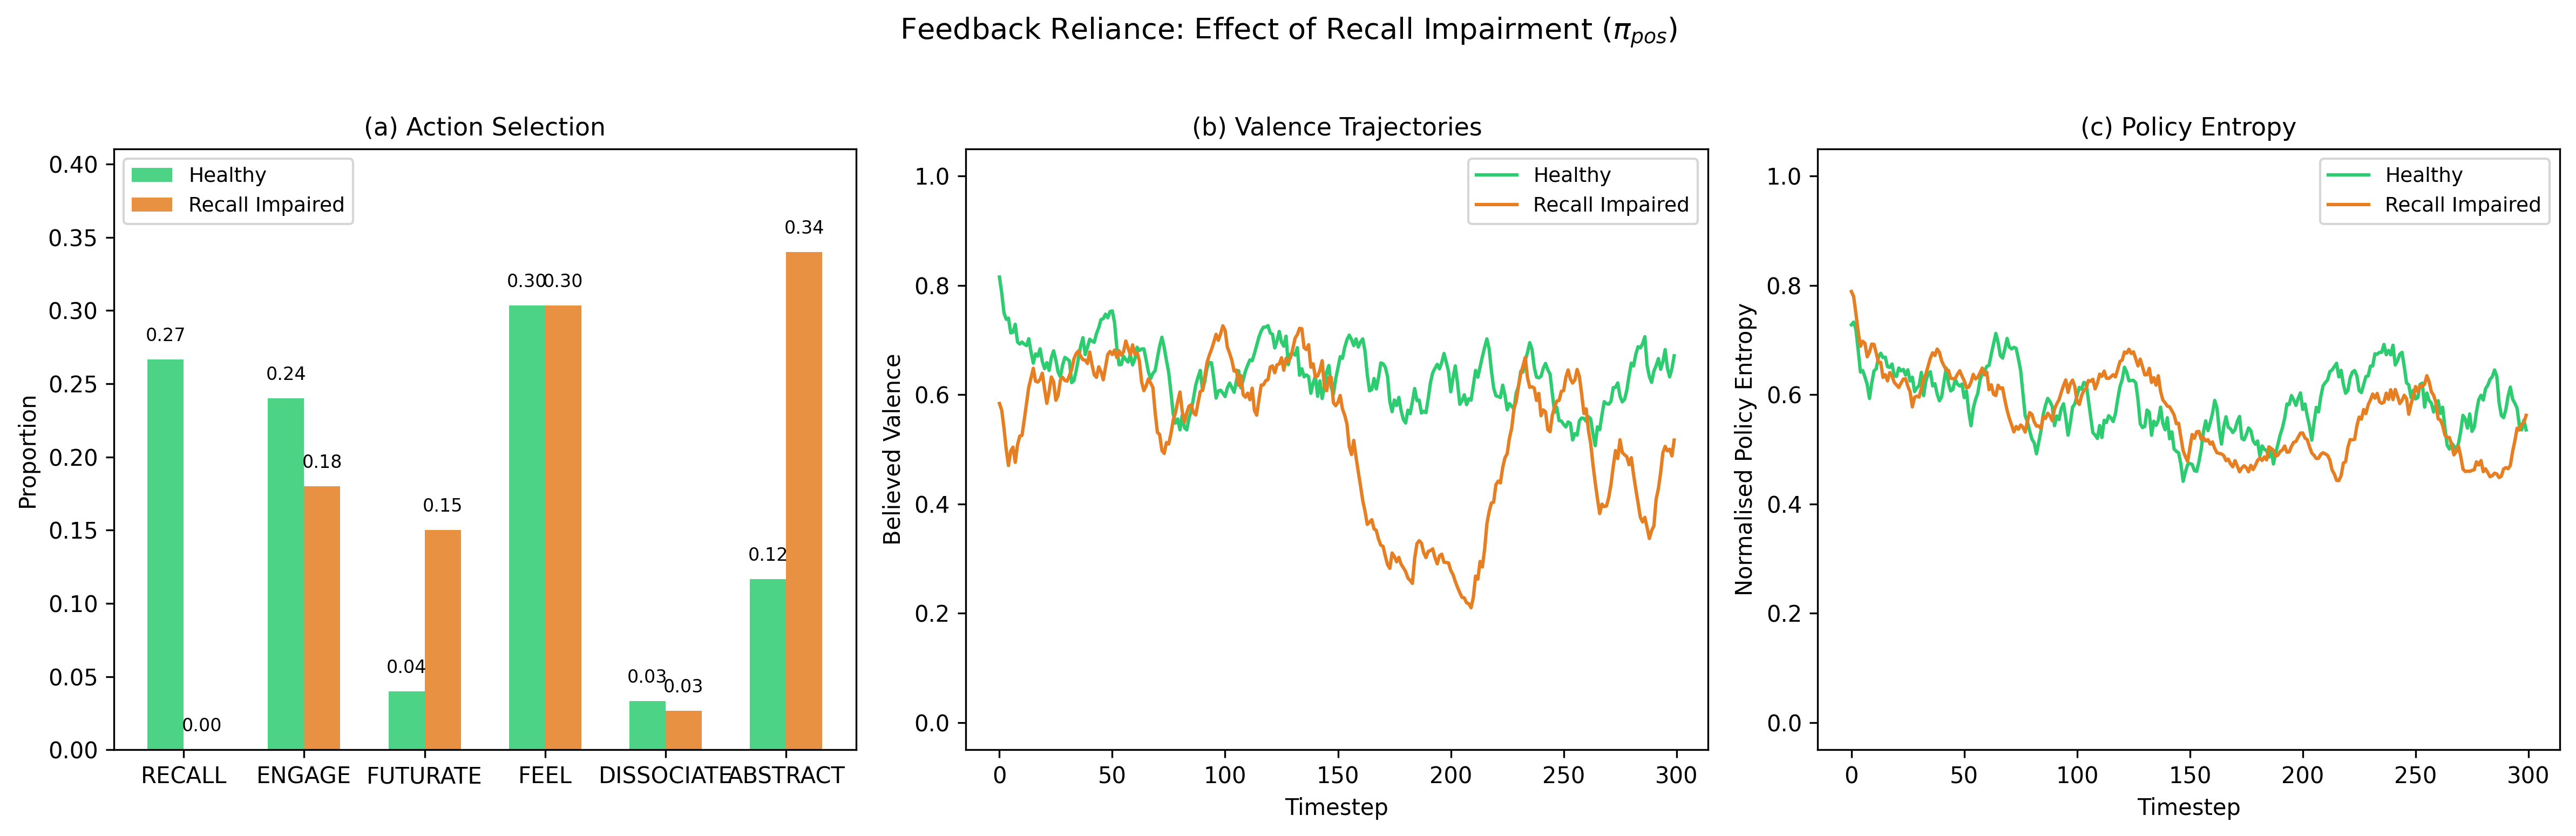
\includegraphics[width=\textwidth]{figures/fig10_feedback_reliance.png}
    \caption{\textbf{Feedback reliance under recall impairment.} Both profiles share $c_{\text{scale}} = 1.0$, $K = 8$, $\omega_e = 5.0$, $\gamma = 16$; they differ only in $\pi_{\text{pos}}$ (5.0 vs 0.2). (a) Action proportions: the recall-impaired agent's RECALL drops from 27\% to $<$1\%, with compensatory ABSTRACT (34\%), FEEL (30\%), ENGAGE (18\%), and FUTURATE (15\%). (b) Valence trajectories: recall impairment reduces mean valence despite intact reward sensitivity. (c) Policy entropy: the recall-impaired agent is less decisive.}
    \label{fig:feedback_reliance}
\end{figure}


\section{Future-Oriented Framing: Reactive Planning}\label{sec:future}

\subsection{Mechanism of FUTURATE}\label{sec:futurate_mechanism}

The FUTURATE policy redistributes precision toward anticipated future states. $\mathbf{B}_v^{\textsc{futurate}}$ pulls valence toward the solution state $K{-}1$ (50\% pull strength), modelling the generation of a highly precise prospective counterfactual. The energy cost is moderate ($-0.5$ per step), reflecting the metabolic expense of prospective simulation. $\mathbf{B}_f^{\textsc{futurate}}$ is 90\% absorbing: once the agent enters future-oriented framing, narrative inertia keeps it there.

The EFE profile of FUTURATE is distinctive: it has the \emph{lowest} valence risk (because the $\mathbf{B}_v$ pull maximally aligns predicted observations with preferences) but the \emph{highest} energy risk (because of the metabolic cost). This tension between valence benefit and energy cost creates a natural brake on FUTURATE selection.

\subsection{Triggered by High Prediction Error}\label{sec:futurate_trigger}

When the agent's beliefs are far from preferred (high VFE), all policies have large risk terms. However, FUTURATE has the largest risk \emph{reduction} because $\mathbf{B}_v^{\textsc{futurate}}$ pulls most strongly toward the preferred state. The standard softmax $\pi(a) \propto \exp(-\gamma \cdot G(a))$ naturally selects FUTURATE when VFE is high, not as a heuristic but as an emergent consequence of the EFE decomposition.

Simulation evidence confirms this (Figure~\ref{fig:framing_dynamics}b, f). Mean VFE conditioned on selected action shows that FUTURATE is preferentially selected at higher-VFE timesteps than RECALL or ENGAGE. The VFE--$\pi(\text{FUTURATE})$ correlation is monotonically positive in healthy and manic agents, and flat in depressive agents (consistent with anhedonia rendering all policies similarly valued).

\subsection{Shorter Behavioural Horizons}\label{sec:short_horizon}

FUTURATE's energy cost creates a natural brake via EFE. After one to two steps of FUTURATE, the predicted interoceptive observation enters the ``depleted'' range, which increases the energy-modality risk term. The softmax shifts away from FUTURATE, producing short, reactive planning bursts rather than sustained commitment.

Simulation evidence (Figure~\ref{fig:framing_dynamics}c) confirms this brake. The healthy agent selects FUTURATE at a low but non-zero rate ($\approx 6\%$), producing short reactive planning bursts that are quickly terminated by the energy cost. RECALL, FEEL, and ENGAGE cycle with short run lengths ($\approx 1.6$, $1.3$, and $1.2$ timesteps, respectively), and FUTURATE bursts are similarly brief ($\approx 1.2$ steps). In the manic agent, strongly amplified reward sensitivity ($c_{\text{scale}} = 6.0$) overrides the energy brake, producing FUTURATE run lengths of $\approx 2.7$ timesteps---the longest of any action, with 63\% selection rate. The contrast is mechanistically transparent: RECALL has minimal energy cost and FEEL actively restores energy, while FUTURATE's energy cost provides an inherent self-limiting mechanism that is overcome only by pathological reward amplification. In the healthy agent, FUTURATE is a minor but adaptive component of the temporal repertoire; in the manic agent, it becomes the dominant and self-reinforcing planning mode.

\subsection{Frame Beliefs and Temporal Orientation}\label{sec:frame_beliefs}

The posterior frame belief $q(f \mid o)$, obtained by marginalising the full posterior over valence and energy, provides a direct readout of the agent's believed temporal orientation. Healthy agents show frame allocation dominated by present ($\approx 0.47$) with balanced past and future ($\approx 0.22$ and $\approx 0.32$), reflecting the adaptive RECALL--FEEL--ENGAGE--FUTURATE cycle (Figure~\ref{fig:framing_dynamics}a). The three clinical phenotypes show qualitatively distinct profiles: depressive agents show past-dominated frame belief ($\approx 0.36$) reflecting the RECALL-dominated ruminative processing style driven by the habit prior (\S\ref{sec:gen_model}), with present and future frame beliefs roughly equal ($\approx 0.32$ each); manic agents show dominant future-frame belief ($\approx 0.68$) from FUTURATE dominance (the forward-projected optimism characteristic of mania); and healthy agents maintain the most balanced temporal profile.

\begin{figure}[htbp]
    \centering
    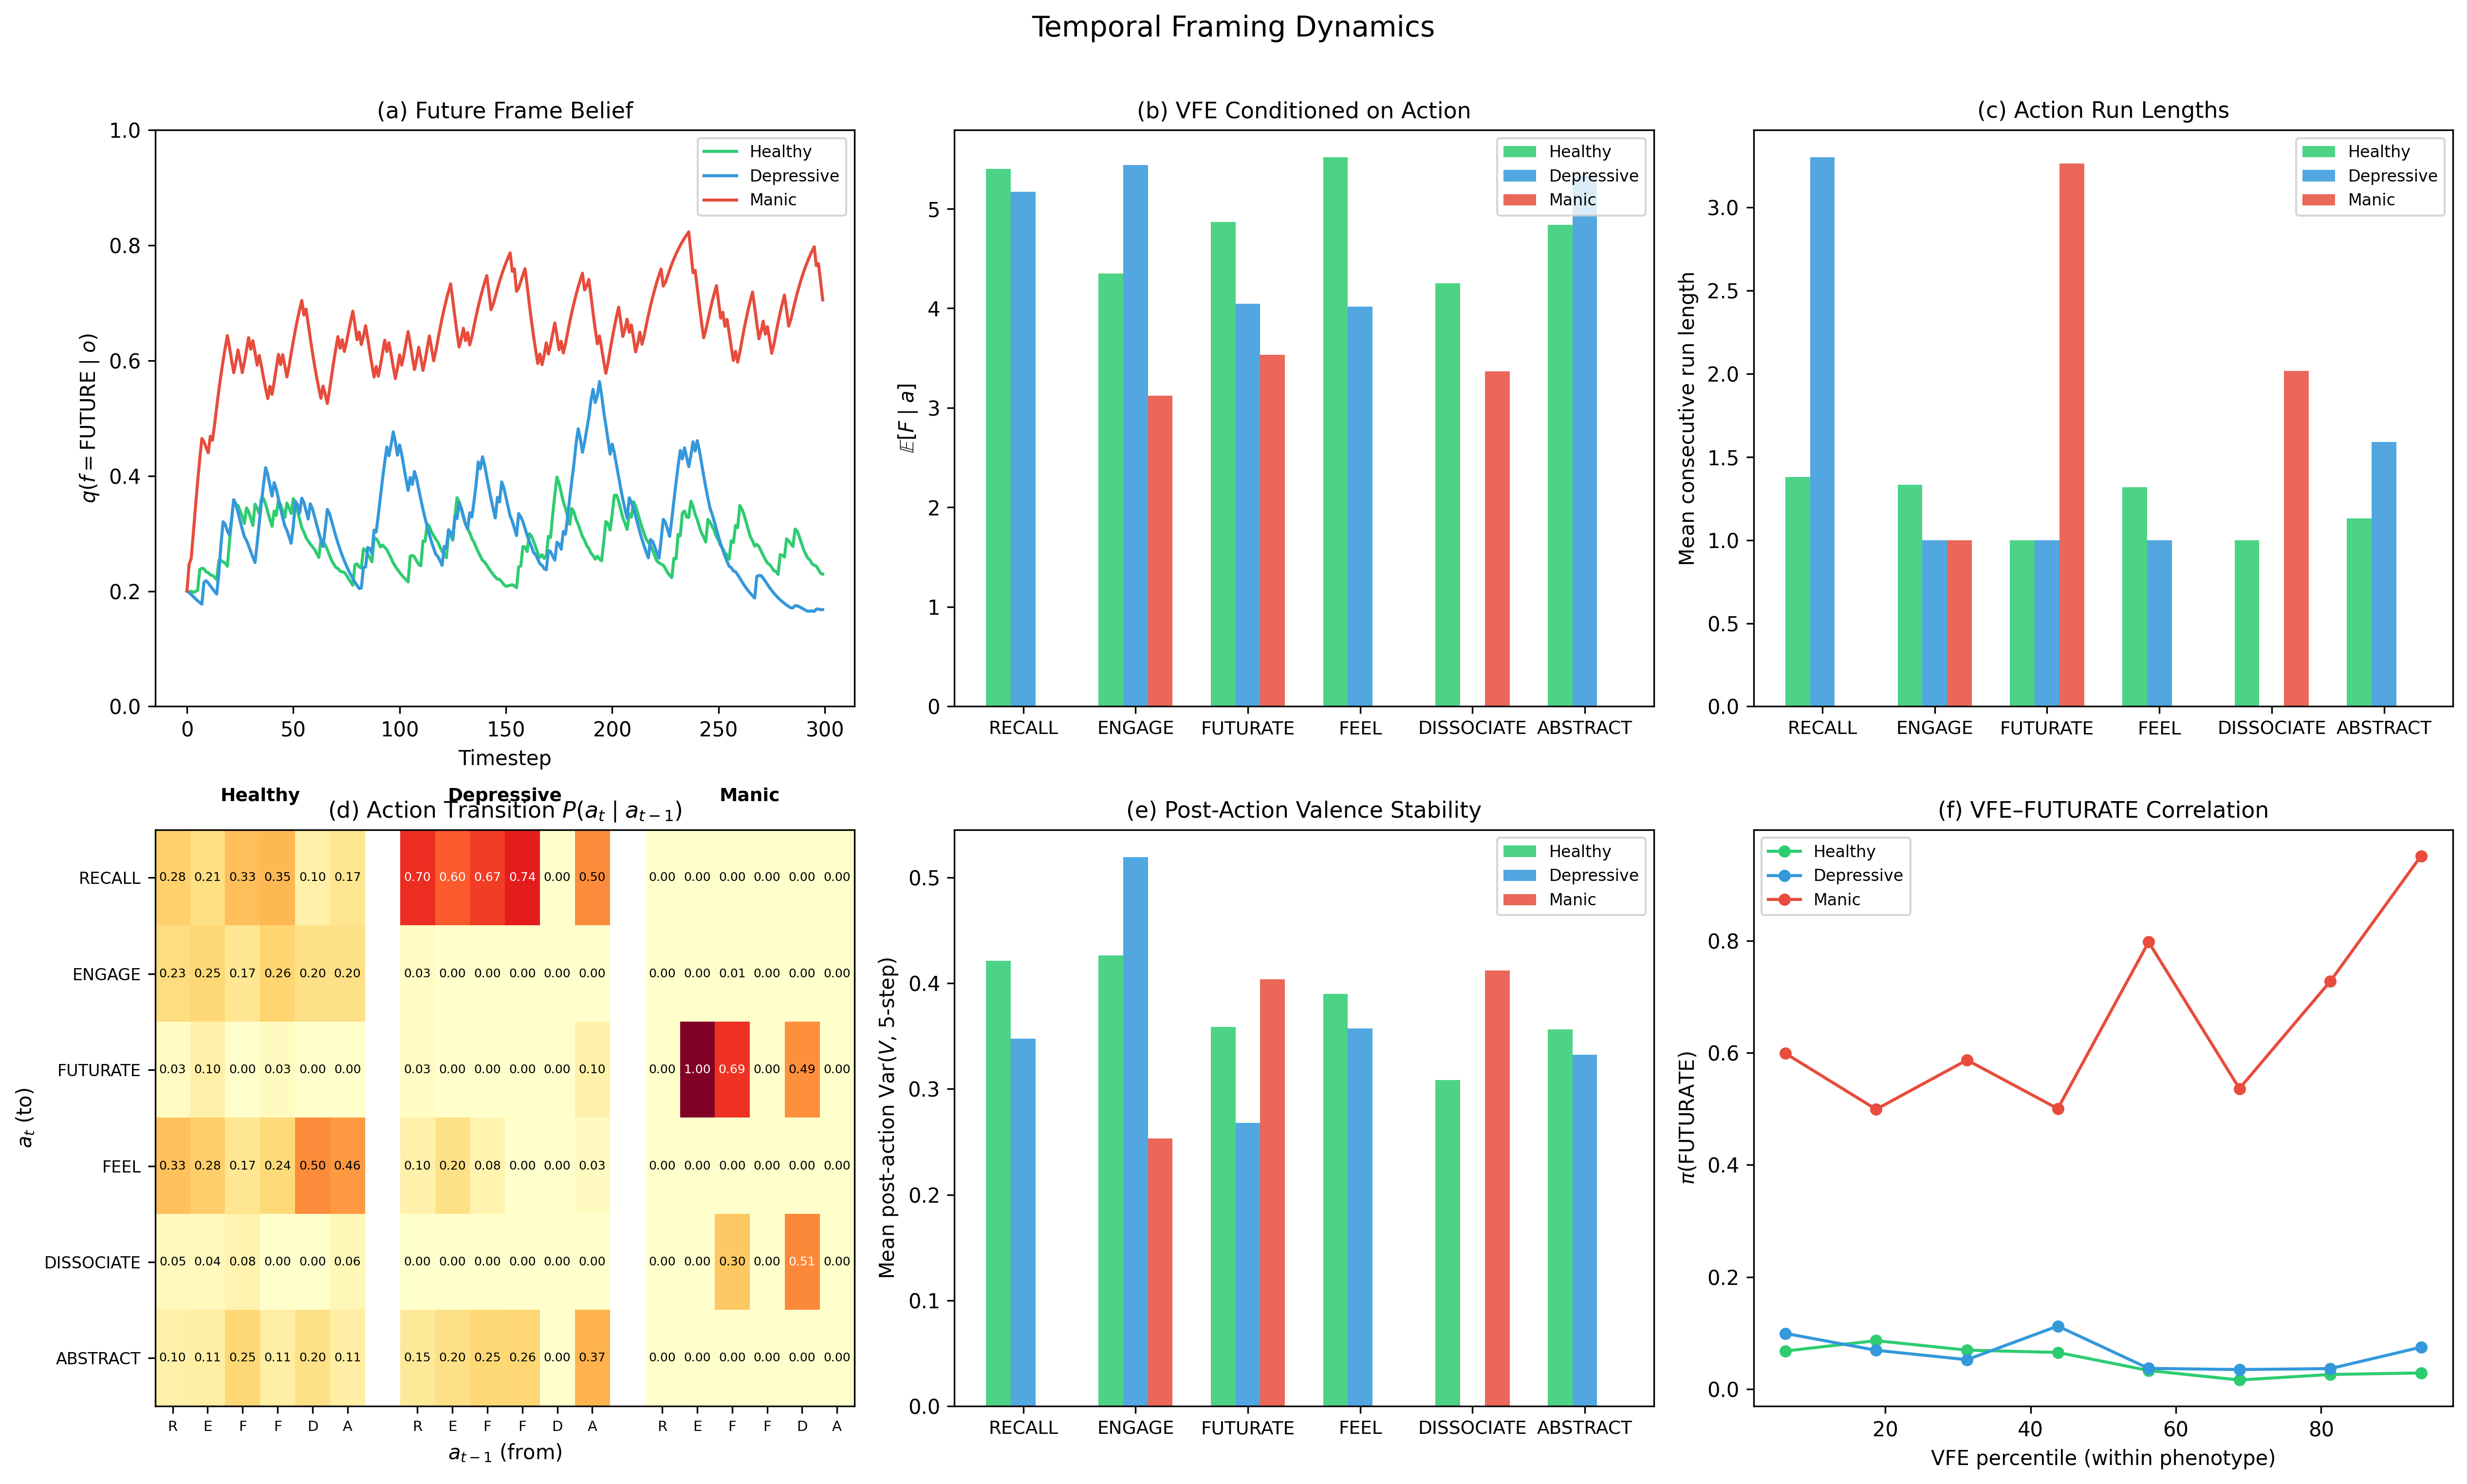
\includegraphics[width=\textwidth]{figures/fig11_framing_dynamics.png}
    \caption{\textbf{Temporal framing dynamics.} (a) Future frame belief $q(f{=}\textsc{future} \mid o)$ over time per phenotype, demonstrating differential temporal orientation. (b) Mean VFE conditioned on selected action: FUTURATE is preferentially selected at higher-VFE timesteps. (c) Mean action run length: FUTURATE runs are shorter than RECALL runs, reflecting reactive planning. (d) Action transition matrices $P(a_t \mid a_{t-1})$ per phenotype, showing the RECALL$\to$ENGAGE pipeline in healthy agents. (e) Post-action valence stability: 5-step rolling variance following each action; RECALL produces lower variance in healthy agents. (f) Binned VFE vs $\pi(\text{FUTURATE})$: monotonic positive relationship in healthy and manic agents, flat in depressive.}
    \label{fig:framing_dynamics}
\end{figure}


\section{Chronic Stress as Maladaptive Temporal Fixation}\label{sec:chronic_stress}

\subsection{Self-Regulation Versus Self-Amplification}\label{sec:self_reg}

The emotion--action--inference loop (\S\ref{sec:loop}) admits two dynamical regimes. Under \emph{self-regulation}, the loop is homeostatic: high VFE triggers corrective action selection, which reduces prediction error; positive $v_{\text{action}}$ reinforces precision on the corrective trajectory \citep{joffily2013emotional}. This is the healthy default, in which prediction errors are informative signals that improve the model.

Under \emph{self-amplification}, the loop becomes pathological. When temporal framing locks into a single mode, precision on that mode's prediction errors increases, and the agent cannot update away from the locked frame. Chronic stress represents the self-amplifying pathology of temporal framing.

\subsection{The Pathological Cycle}\label{sec:pathological_cycle}

We introduce a ``stressed'' profile characterised by four concurrent perturbations from the healthy baseline: very high environmental volatility ($0.9$ vs $0.3$), elevated reward sensitivity ($c_{\text{scale}} = 2.0$ vs $1.0$), stress-impaired interoception ($\omega_e = 0.5$ vs $5.0$), and reduced positive-belief precision ($\pi_{\text{pos}} = 2.5$ vs $5.0$). The interoceptive impairment is clinically grounded: chronic stress is associated with reduced interoceptive accuracy \citep{barrett2017theory, seth2016interoceptive}.

These perturbations interact through the EFE decomposition in three reinforcing ways. First, impaired interoception ($\omega_e = 0.5$) blurs the agent's $\mathbf{A}_{\text{int}}$ matrix, reducing the energy-modality risk term that would normally deter FUTURATE selection and simultaneously eliminating the interoceptive differentiation that supports FEEL; in effect, both the brake and the body-awareness pathway are disabled. Second, elevated reward sensitivity ($c_{\text{scale}} = 2.0$) amplifies the hedonic preference vectors $\mathbf{C}_{\text{ext}}$ and $\mathbf{C}_{\text{val}}$, increasing the valence-modality risk reduction for FUTURATE; the accelerator is enhanced. Third, under the standard softmax policy selection $\pi(a) \propto \exp(-\gamma \cdot G(a))$, FUTURATE and RECALL naturally enter the policy mix when the brake is disabled and the accelerator is enhanced, producing the rumination-plus-worry pattern.

Once FUTURATE enters the policy mix, its 90\% absorbing frame transition creates narrative inertia, causing the agent to persist in future-oriented framing. Meanwhile, RECALL's strong past-frame transition ($\approx 70\%$) creates a complementary backward pull. The volatile environment keeps violating the agent's precise predictions from both directions, producing chronic positive $\Delta F$ (increasing VFE). DISSOCIATE fills the gaps between directed temporal processing, its diffuse frame transition spreading temporal belief across all horizons. This creates the self-amplifying cycle: directed temporal processing (RECALL + FUTURATE) produces precise predictions, which the environment violates, producing negative $v_{\text{model}}$, which elevates VFE and further favours these over present-oriented engagement (\S\ref{sec:futurate_trigger}).

\subsection{Temporal Dysregulation Pattern}\label{sec:temporal_dysreg}

The stressed agent's posterior frame belief shows a characteristic pattern of future-dominated temporal fixation: dominant \textsc{future} ($0.72$ vs $0.30$ in healthy), with severely depleted \textsc{present} ($0.19$ vs $0.48$) and reduced \textsc{past} ($0.09$ vs $0.22$). The stressed agent is drawn overwhelmingly toward future framing at the expense of present engagement (Figure~\ref{fig:chronic_stress}a). The action profile confirms this: FUTURATE dominates (71\%), supplemented by DISSOCIATE (20\%) and ABSTRACT (3\%), while present-oriented ENGAGE collapses (4\%) and both RECALL and FEEL disappear ($\approx$1\%).

This pattern of dominant future framing with depleted present engagement is the computational signature of anxious prospective simulation---the ``worry'' component of chronic stress \citep{berg2022rumination}. FUTURATE dominance reflects the interaction of reward hypersensitivity ($c_{\text{scale}} = 2.0$) with impaired interoception ($\omega_e = 0.5$) under very high volatility (0.9): the energy brake is disabled (the agent cannot predict depletion) while the hedonic accelerator is enhanced (amplified $\mathbf{C}_{\text{val}}$ increases FUTURATE's risk reduction). The near-absence of RECALL ($\approx 1\%$) reflects the reduced $\pi_{\text{pos}} = 2.5$ ($\alpha \approx 0.62$, recall target at $\approx 57\%$ of max valence), which makes RECALL EFE-uncompetitive against the strong FUTURATE pull. The presence of DISSOCIATE (20\%) reflects periods of temporal unmooring---disengagement from directed processing---consistent with the dissociative episodes reported under chronic stress. Crucially, FEEL is entirely absent: the stressed agent's impaired interoception renders interoceptive processing uninformative, blocking the body-awareness pathway that healthy agents use for self-regulation.

\subsection{Persistent Backward Negative Valence}\label{sec:backward_negative}

The stressed agent's backward valence $v_{\text{model}} = \tanh(-\Delta F / \tau)$ is persistently more negative than the healthy agent's (Figure~\ref{fig:chronic_stress}b). The mechanism is precise: the volatile environment keeps violating the agent's predictions (producing positive $\Delta F$), so the backward channel, which evaluates how well past predictions matched observations, is persistently negative.

FUTURATE exacerbates this effect. By pulling beliefs toward the solution state, FUTURATE creates \emph{precise predictions about positive future outcomes} that the volatile environment then violates, amplifying $\Delta F$. The backward negative valence is therefore not a belief about the past being bad, but a \emph{signal} that the model's fit to recent observations is deteriorating, a signal amplified by the very mechanism (FUTURATE) that the agent uses to cope.

\subsection{Channel Decomposition}\label{sec:channel_decomp}

The stressed agent's valence channel decomposition reveals the full temporal structure of chronic stress (Figure~\ref{fig:chronic_stress}c). The reward channel ($v_{\text{reward}} = -0.12$) is the dominant driver of negative valence: FUTURATE's $\mathbf{B}_v$ pull (50\% toward max valence) elevates expected utility $\mathbb{E}[U]$, but the highly volatile environment delivers observations below expectation ($U < \mathbb{E}[U]$), producing persistent negative hedonic surprise. The backward channel ($v_{\text{model}} = +0.01$) is only mildly positive, as the high volatility produces roughly symmetric prediction errors. The action channel ($v_{\text{action}} = +0.06$) remains positive: the agent keeps finding ``better'' policies under high VFE (policy improvement is easy when the current policy is poor), but the improvement is ephemeral because the environment keeps changing.

This pattern of strongly negative reward valence alongside persistent forward positivity is the computational signature of \emph{frustrated forward projection}: the agent is trapped in optimistic planning that systematically fails to deliver, producing the chronic hedonic disappointment characteristic of stressed overmentalising.

\begin{figure}[htbp]
    \centering
    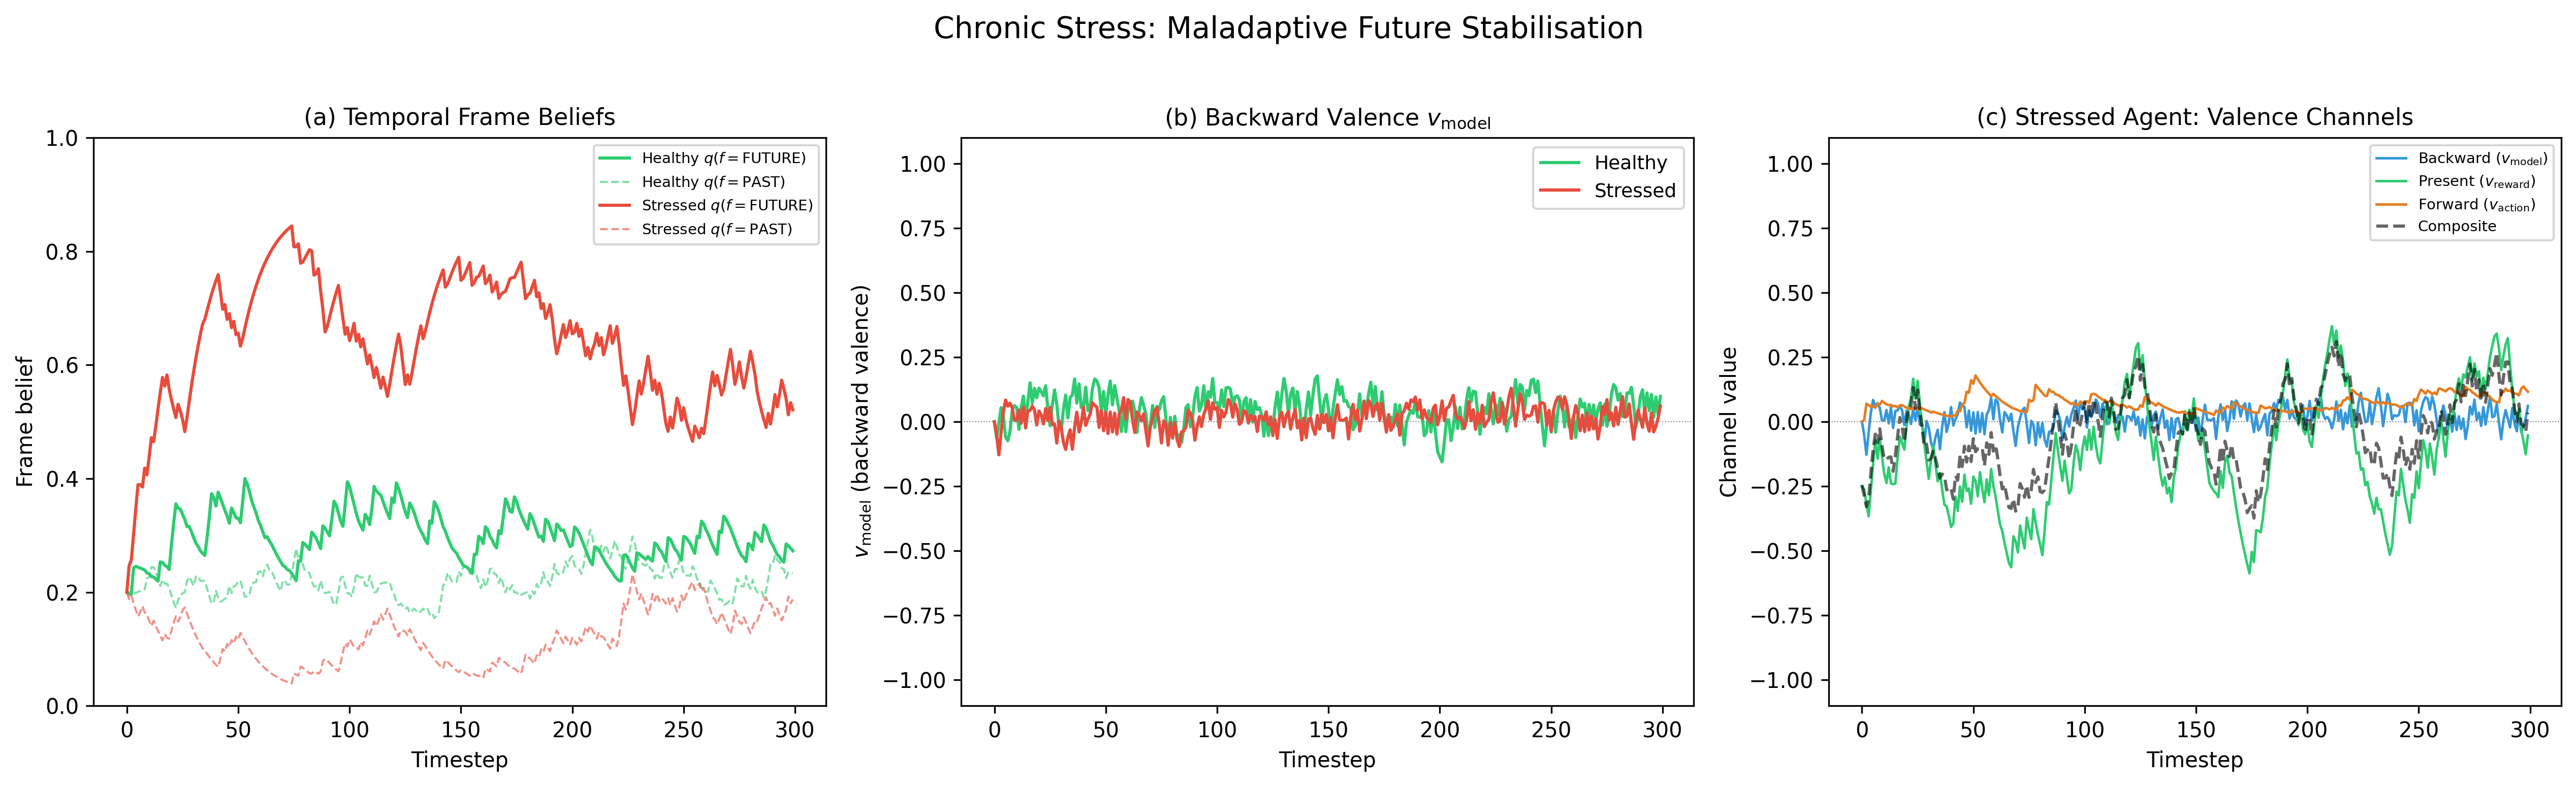
\includegraphics[width=\textwidth]{figures/fig12_chronic_stress.png}
    \caption{\textbf{Chronic stress as maladaptive temporal fixation.} Stressed profile ($\pi_{\text{pos}} = 2.5$, $c_{\text{scale}} = 2.0$, $\omega_e = 0.5$, volatility $= 0.9$) vs healthy ($\pi_{\text{pos}} = 5.0$, $c_{\text{scale}} = 1.0$, $\omega_e = 5.0$, volatility $= 0.3$); $K{=}8$, $\gamma = 16$ shared. (a)~Frame beliefs: the stressed agent shows dominant FUTURE ($0.72$ vs $0.30$) with depleted PRESENT ($0.19$ vs $0.48$) and reduced PAST ($0.09$ vs $0.22$), the signature of anxious prospective fixation. (b)~Backward valence $v_{\text{model}}$: more variable in the stressed agent from high volatility. (c)~Valence channel decomposition for the stressed agent: reward channel ($v_{\text{reward}} = -0.12$) drives composite valence negative via frustrated forward projection, action channel showing persistent positive bursts ($v_{\text{action}} = +0.06$).}
    \label{fig:chronic_stress}
\end{figure}


\section{Discussion}\label{sec:discussion}

\subsection{Temporal Aiming as a Unified Theory}\label{sec:unified_theory}

This paper has formally proposed what has been implicit in the active inference literature but never unified in a single account: the VFE/EFE distinction provides a natural temporal taxonomy of emotion. Variational free energy concerns beliefs about what \emph{has happened} and generates backward-oriented affect (regret, guilt, pride, gratitude). Expected free energy concerns expectations about what \emph{will happen} and generates forward-oriented affect (hope, fear, anxiety, anticipation). The rate of change at the current moment generates present-oriented affect (joy, anger, surprise). Transitional emotions (relief, disappointment) arise from comparing current VFE with prior EFE predictions.

Counterfactual temporal framing is the \emph{mechanism} by which agents actively navigate this temporal structure. Different from \citet{hinrichs2025temporal}, who addressed temporal aiming in dyadic geometric hyperscanning, we have addressed the single-agent computational mechanism: temporal framing as precision redistribution across temporal horizons, naturally selected by EFE minimisation.

\subsection{Temporal Framing as a General Mechanism}\label{sec:general_mechanism}

Temporal framing is not specific to pathology. Healthy agents \emph{use} all six temporal modes for adaptive regulation: RECALL stabilises affect (creating a floor under valence), FEEL manages the energy budget through interoceptive processing, ENGAGE maintains environmental coupling, FUTURATE provides reactive planning bursts (responding to high prediction error, $\approx 7\%$ of timesteps), ABSTRACT provides a secondary hedonic pathway, and DISSOCIATE provides brief temporal unmooring during transitions. The moderate energy cost of FUTURATE ($-0.5$) provides a self-limiting brake that keeps it adaptive rather than dominant. Pathology arises not from temporal framing itself but from the failure of its balancing mechanisms: when the brake is disabled (impaired interoception) and the accelerator is strongly amplified ($c_{\text{scale}} = 6.0$), FUTURATE runs unchecked (mania); when the accelerator is enhanced and the environment is volatile, forward projection dominates with frustrated reward (chronic stress); when hedonic sensitivity is asymmetric ($c_{\text{pos}} \ll c_{\text{neg}}$) and a ruminative habit prior locks the agent onto RECALL, the temporal repertoire constricts onto past-directed processing (depression).

\subsection{Metastability as Health}\label{sec:metastability}

A key insight emerging from the simulations is that health is not a particular temporal configuration but the \emph{capacity to transition between configurations}. The healthy agent's defining characteristic is not its specific action mix (FEEL~29\%, RECALL~23\%, ENGAGE~23\%, ABSTRACT~13\%, FUTURATE~7\%, DISSOCIATE~3\%) but its high switching rate and short mean run length. Five distinct temporal modes are actively deployed, none dominating for more than a few consecutive steps. This is metastability in the dynamical systems sense: the agent visits multiple attractor basins without becoming trapped in any one.

Pathology, on this account, is \emph{stickiness}. The manic agent shows the longest runs (FUTURATE mean $\approx 2.7$ steps, 64\% selection rate), reflecting persistent lock-in to forward projection. The depressive agent shows severe mode constriction of a different kind: the habit prior (E~vector, \S\ref{sec:gen_model}) locks RECALL at 66\%, supplemented by ABSTRACT (18\%) as the only non-penalised escape route, while FUTURATE, ENGAGE, and FEEL are all suppressed below 8\%. Both pathologies reduce the agent's effective temporal repertoire, but through different mechanisms: mania through absorptive narrative inertia (FUTURATE's 90\% frame self-transition) combined with amplified reward sensitivity ($c_{\text{scale}} = 6.0$), depression through habitual ruminative recall that overrides EFE-optimal policy selection \citep{nolenhoeksema2008rethinking}.

This framing has clinical implications. An agent locked into ENGAGE during a crisis is not pathological---context-appropriate dominance of a single mode is adaptive. The pathology lies in the inability to \emph{exit} that mode when context changes. In depression, the habit prior makes RECALL ``sticky'' in a way that EFE minimisation alone cannot correct: the agent is trapped not by the EFE landscape but by the habitual override of it. Therapeutic interventions, on this view, should target the switching mechanism rather than any particular mode: behavioural activation targets the habit prior by forcing action diversity, while cognitive therapy targets the escape-route aversion ($E_{\textsc{futurate}} < 0$, $E_{\textsc{abstract}} < 0$) that prevents the agent from engaging future-oriented processing. Restoring the ability to transition between temporal orientations is more fundamental than correcting the balance between them.

\subsection{Connection to Attention-as-Precision}\label{sec:attention_connection}

\citet{feldman2010attention} established that attention is precision weighting on prediction errors. Our framework extends this to the temporal domain: \emph{temporal attention} is precision weighting on temporal horizons. The $\mathbf{B}_{\text{frame}}$ matrices function as temporal attention operators, and action selection in the temporal framing domain amounts to deciding \emph{where in time} to attend. This connects temporal framing to the broader predictive processing literature on selective attention, suggesting that spatial attention (``where to look'') and temporal attention (``when to think about'') are instances of the same precision-weighting mechanism applied to different dimensions of the generative model.

\subsection{Mood Versus Emotion Timescales}\label{sec:mood_emotion}

\citet{hesp2021deeply} distinguished two timescales in the affect hierarchy: M4 (emotion), operating within-trial as fast precision dynamics, and M5 (mood), operating cross-trial as slow valence state inference. Temporal framing operates at the \emph{interface} between these timescales. Individual frame selections are M4 phenomena, reflecting fast, within-trial decisions about temporal orientation driven by current EFE. Sustained frame biases are M5 phenomena, reflecting slow, cross-trial tendencies toward particular temporal orientations that encode learned or dispositional patterns.

We implement the M5 layer as a \emph{hierarchical POMDP} over the positive-belief precision parameter $\pi_{\text{pos}}$. The mood level maintains a categorical belief $q(\mu)$ over $N_\mu = 8$ discretised mood states $\mu \in \{0.5, 1.5, \ldots, 7.5\}$, each corresponding to a value of $\pi_{\text{pos}}$. Every $T_\mu = 50$ emotion-level steps, the mood level performs one cycle of Bayesian inference:

\textbf{Observation.} The mood-level observation is the mean variational free energy (VFE) over the preceding window: $\bar{F} = T_\mu^{-1} \sum_{t' \in \text{window}} F(t')$. This is binned into $N_o^\mu = 5$ categories. The observation model $\mathbf{A}^\mu$ encodes the expectation that higher mood states (higher $\pi_{\text{pos}}$, hence better RECALL effectiveness) produce lower VFE:
\begin{equation}
    P(o^\mu \mid \mu) \propto \exp\!\left( -\frac{(\bar{o}^\mu - \hat{F}(\mu))^2}{2\sigma_A^2} \right), \qquad \hat{F}(\mu) = 4.14 + 0.66\,(1 - \sigma(\mu - 2))
\end{equation}
where $\hat{F}(\mu)$ is the expected VFE given mood state $\mu$ and $\sigma_A = 0.2$.

\textbf{Transition.} The mood-level transition model $\mathbf{B}^\mu$ is near-diagonal (self-transition probability $0.97$, symmetric $\pm 1$ transitions at $0.015$), encoding the empirical observation that mood is highly persistent. All asymmetry in mood drift arises from the VFE evidence, not from built-in bias.

\textbf{Update.} Standard Bayesian filtering:
\begin{align}
    q_{\text{pred}}(\mu) &= \mathbf{B}^\mu\, q(\mu) \\
    q(\mu \mid o^\mu) &\propto P(o^\mu \mid \mu)\, q_{\text{pred}}(\mu)
\end{align}

\textbf{Readout.} The expected $\pi_{\text{pos}}$ under the mood posterior parameterises the emotion-level $\mathbf{B}$ matrices:
\begin{equation}
    \pi_{\text{pos}} = \mathbb{E}_{q(\mu)}[\mu] = \sum_i \mu_i\, q(\mu_i)
\end{equation}

This hierarchical architecture creates self-reinforcing attractor dynamics entirely from Bayesian inference. A healthy agent in a benign environment experiences low VFE, which is consistent with high mood states, maintaining $\pi_{\text{pos}}$ and RECALL effectiveness. Conversely, chronic prediction error (high VFE) shifts the mood posterior toward lower states, weakening RECALL, which further elevates VFE---producing the depressive attractor. Clinical phenotypes thus emerge as stable attractors of the hierarchical mood dynamics rather than being imposed as fixed parameter settings.

The transition from adaptive temporal framing (M4) to chronic temporal fixation (M5) is precisely the self-amplification pathology described in \S\ref{sec:chronic_stress}. We demonstrate this with a stress decay experiment (Figure~\ref{fig:stress_decay_p2}): two agents with identical healthy initial conditions ($\pi_{\text{pos}} = 5.0$) are placed in environments differing only in volatility ($0.3$ vs $0.9$). Over $T = 3000$ steps, the hierarchical mood posterior diverges dramatically: the healthy agent's $\mathbb{E}[\pi_{\text{pos}}]$ drifts upward toward $\approx 7.5$ (positive attractor), while the stressed agent's posterior crashes downward through the sigmoid knee at $\pi_{\text{pos}} = 2$, settling near $\approx 0.8$---well below the threshold where RECALL effectiveness collapses entirely (panel~c). This divergence arises purely from accumulated VFE evidence at the mood level, without any change to the agent's initial parameter configuration.

\begin{figure}[htbp]
    \centering
    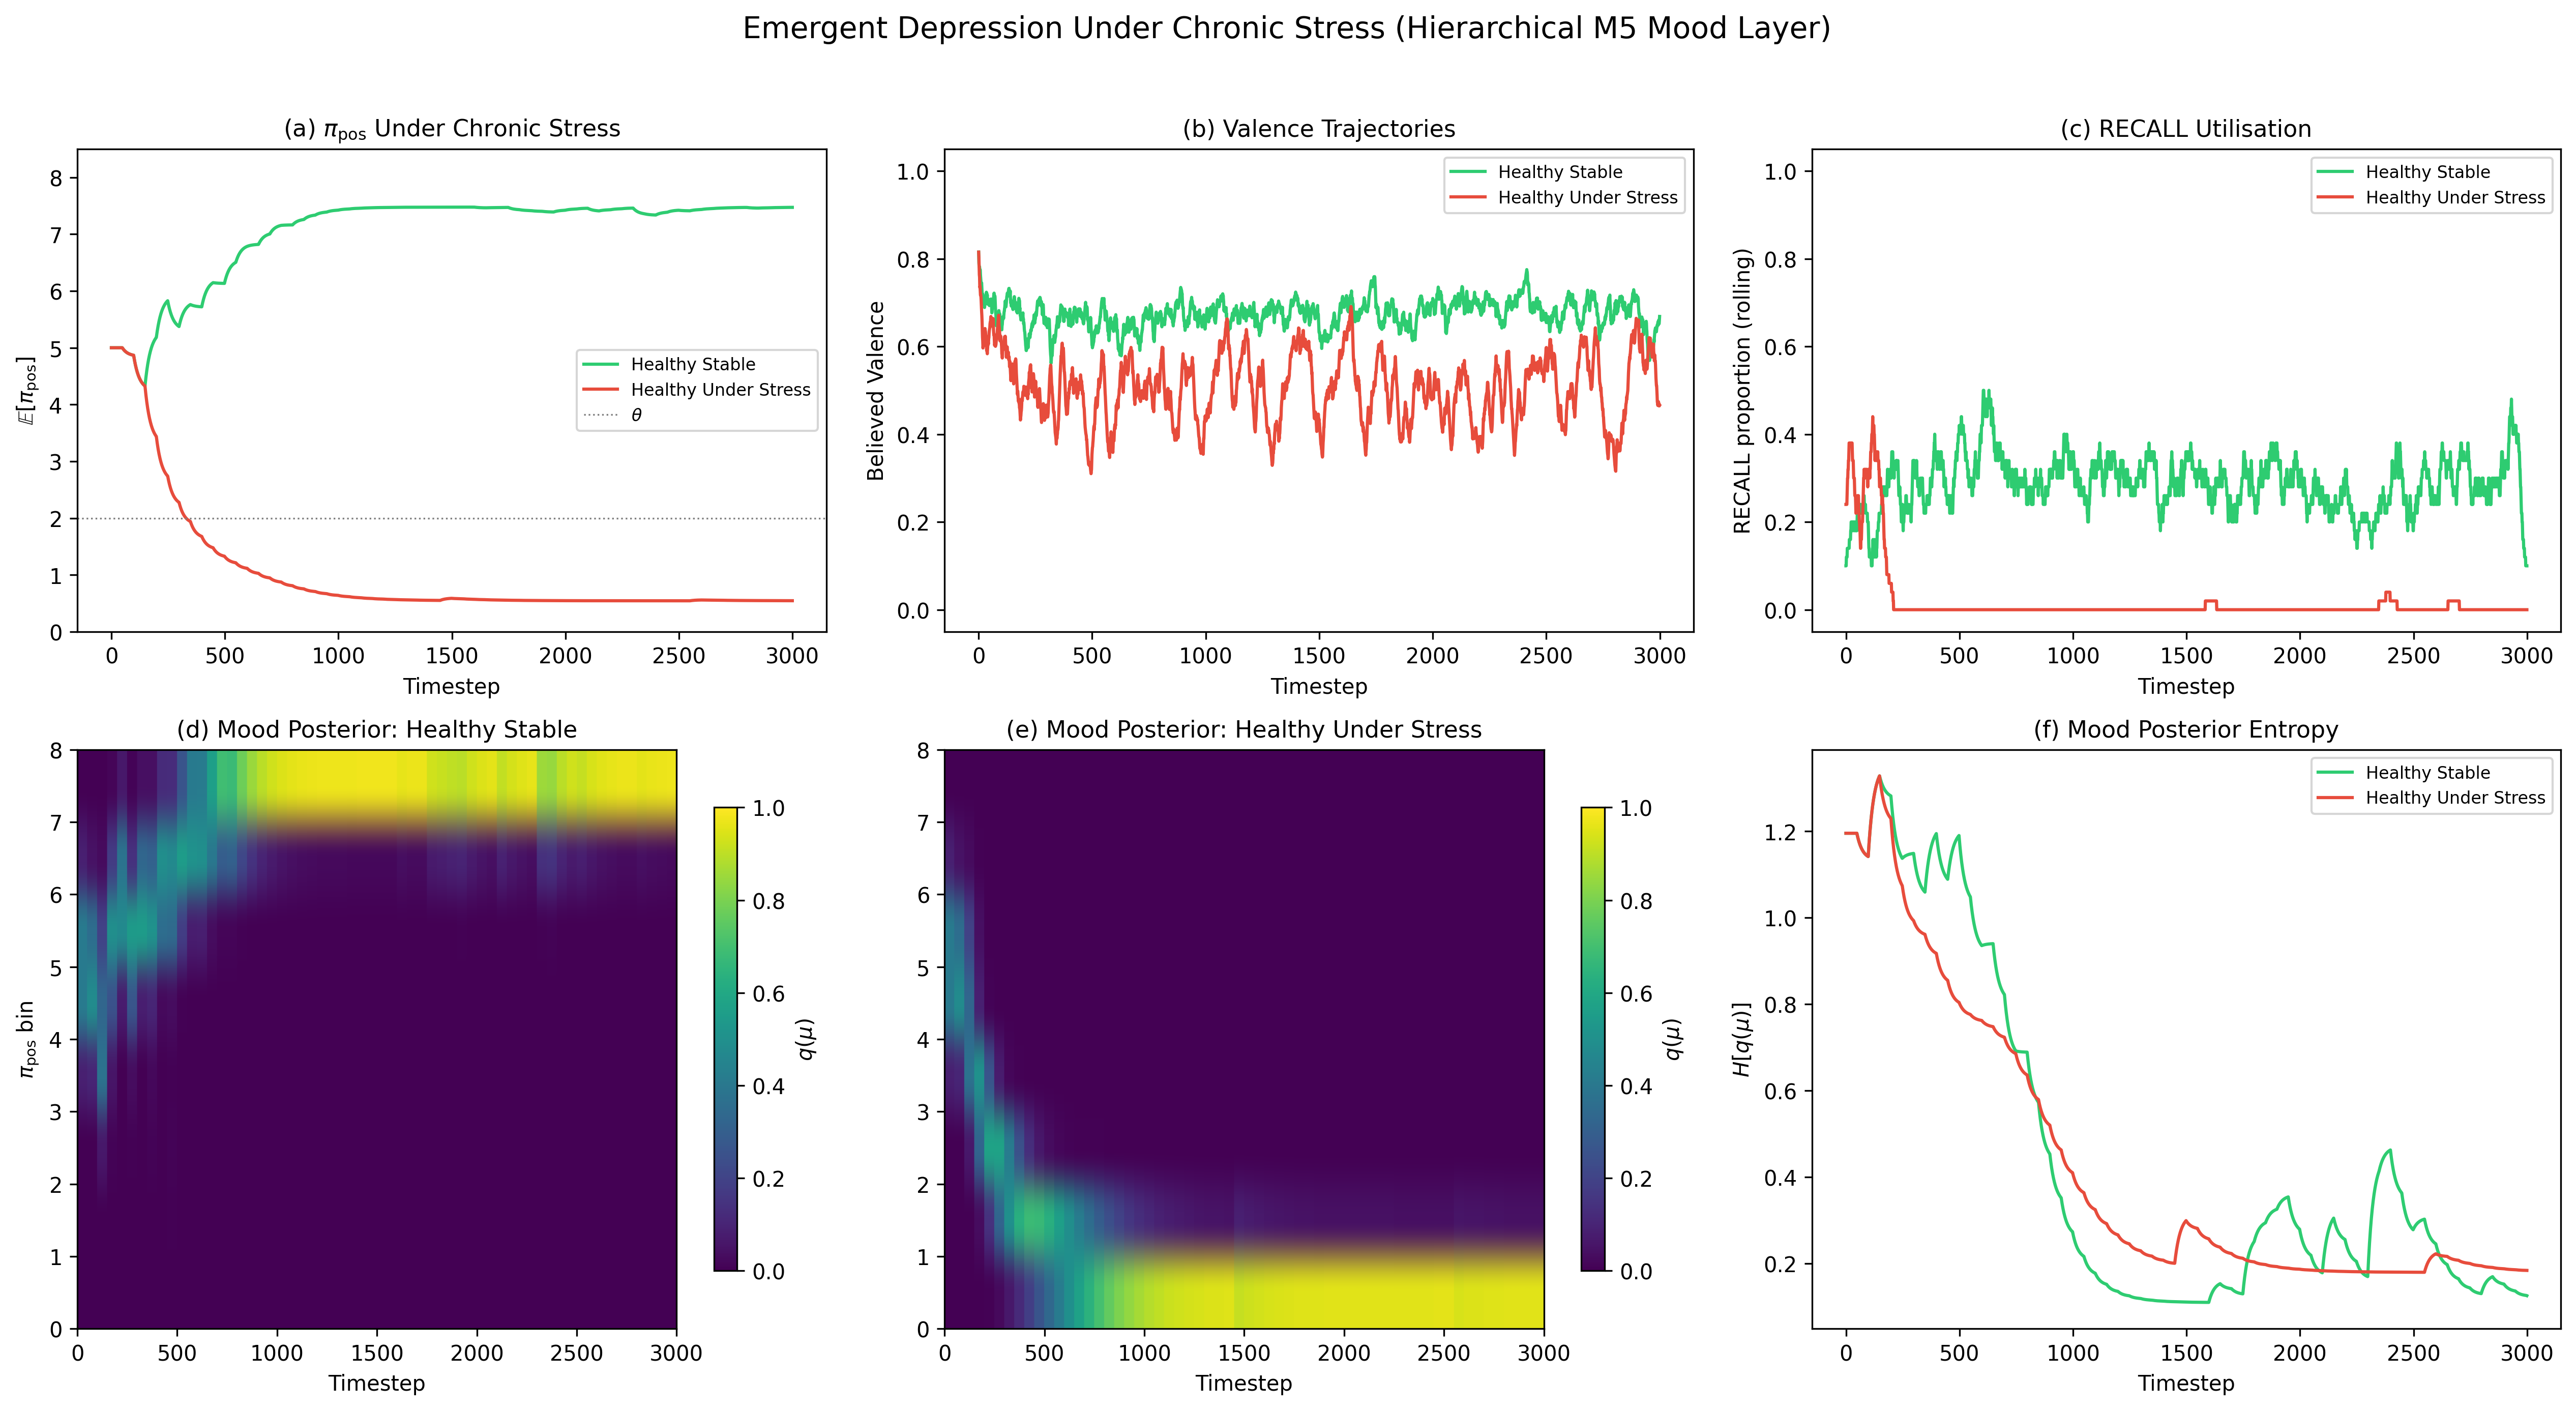
\includegraphics[width=\textwidth]{figures/fig14_stress_decay.png}
    \caption{\textbf{Emergent depression under chronic stress (hierarchical M5 mood layer).} Both agents start with identical healthy parameters ($\pi_{\text{pos}} = 5.0$); the only difference is environmental volatility ($0.3$ vs $0.9$). (a)~$\mathbb{E}[\pi_{\text{pos}}]$ trajectories diverge as the mood posterior shifts. (b)~Valence diverges. (c)~RECALL utilisation. (d--e)~Mood posterior heatmaps show the healthy agent concentrating at high $\mu$ while the stressed agent diffuses toward lower states. (f)~Mood posterior entropy. $T = 3000$.}
    \label{fig:stress_decay_p2}
\end{figure}

\subsection{Relationship to Bipolar Disorder}\label{sec:bipolar_connection}

The same framework can model bipolar disorder as pathology of energy $\times$ interoception $\times$ backward precision, where clinical phenotypes emerge from parameter variation along four dimensions ($\pi_{\text{pos}}$, $K$, $\omega_e$, $c_{\text{scale}}$). The present paper provides the \emph{general temporal mechanism} that bipolar disrupts. The manic phenotype ($\pi_{\text{pos}} = 1.5$, $c_{\text{scale}} = 6.0$, $\omega_e = 0.5$, volatility $= 0.15$) is characterised by low backward-looking positive-belief precision combined with strongly amplified reward processing in a subjectively stable environment: RECALL is insufficiently grounding ($\alpha_{\text{recall}} = 0.38$, and the bidirectional target at $\approx 43\%$ of max valence provides only weak positive pull), so the agent defaults to FUTURATE (64\% selection rate) as the dominant affective regulation strategy, supplemented by DISSOCIATE (35\%) during periods of temporal unmooring. The low environmental volatility captures the grandiose certainty characteristic of mania: the manic agent perceives its environment as predictable, allowing precise forward projections to succeed ($v_{\text{model}} \approx 0$) even as energy depletes catastrophically (mean energy $= 0.22$). This captures the clinical observation that manic optimism is forward-projected rather than backward-grounded \citep{johnson2012behavioral, alloy2010role}. The strongly amplified $c_{\text{scale}} = 6.0$ produces composite valence ($V = +0.11$) comparable to the healthy baseline ($+0.13$), reflecting the elevated hedonic tone characteristic of mania despite energy depletion. Bipolar disorder thus involves pathological \emph{cycling} of temporal frames: manic episodes are locked FUTURATE (aggressive future-oriented framing that depletes energy), crashes are forced FEEL (energy recovery through interoceptive processing), and depressive episodes involve ruminative fixation on the past (RECALL dominance driven by the habit prior, with asymmetric punishment sensitivity maintaining negative reward valence). The depressive and manic profiles share low backward precision but are distinguished by a principled double dissociation: the depressive agent's asymmetric hedonic sensitivity ($c_{\text{pos}} = 0.1$, $c_{\text{neg}} = 2.0$) attenuates positive outcomes while amplifying negative ones, and the habit prior (E~vector) locks the agent into past-directed rumination (RECALL~66\%, \textsc{past} frame~$0.36$), while the manic agent's extreme symmetric hypersensitivity ($c_{\text{scale}} = 6.0$) drives aggressive forward projection \citep{alloy2010role}. Chronic stress, by contrast, involves pathological temporal \emph{fixation}: FUTURATE dominates (71\%) as reward hypersensitivity and impaired interoception disable the energy brake under very high volatility ($0.9$), with DISSOCIATE (20\%) filling the gaps between directed forward projection, and present engagement collapses (4\%). The manic and chronic stress profiles are differentiated not by action proportions (both are FUTURATE-dominant) but by their affective signatures: the manic agent's reward channel is positive ($v_{\text{reward}} = +0.05$, amplified successful forward projection in a stable environment) while the chronic stress agent's is strongly negative ($v_{\text{reward}} = -0.12$, frustrated projection in a volatile environment).

\subsection{Depression as Past-Directed Ruminative Fixation}\label{sec:depression}

Depression can be understood as the pathological locking of temporal framing onto past-directed processing. Two mechanisms jointly produce this pattern: \emph{asymmetric hedonic sensitivity} and the \emph{habit prior} (E~vector).

The depressive agent's hedonic sensitivity is profoundly asymmetric: $c_{\text{pos}} = 0.1$ (severely blunted positive reward) with $c_{\text{neg}} = 2.0$ (amplified punishment sensitivity). This asymmetry shapes the EFE landscape: the risk reduction from moving toward positive states is negligible (flattened $\mathbf{C}_{\text{val}}^{+}$), while the risk associated with negative states is amplified (steep $\mathbf{C}_{\text{val}}^{-}$). From a pure EFE perspective, this asymmetry should drive the agent \emph{away} from negative states via future-oriented planning (FUTURATE) or cognitive reappraisal (ABSTRACT)---the agent should escape, not dwell. Indeed, without the habit prior, the asymmetric agent shows elevated FUTURATE and ABSTRACT selection.

The habit prior resolves this paradox. The E~vector $[10, 0, -1, 0, 0, -1]$ encodes a strong habitual bias toward RECALL ($E_{\textsc{recall}} = 10$) with aversion to the EFE-optimal escape routes ($E_{\textsc{futurate}} = E_{\textsc{abstract}} = -1$). This override produces the characteristic depressive profile: RECALL dominates at 66\%, supplemented by ABSTRACT (18\%) as the only non-penalised cognitive route, with FUTURATE (8\%), FEEL (7\%), ENGAGE (1\%), and DISSOCIATE ($<$1\%) effectively suppressed. The frame posterior reflects this: \textsc{past} is dominant ($0.36$) with \textsc{present} and \textsc{future} roughly equal ($\approx 0.32$ each)---a past-oriented temporal fixation.

This profile captures three key features of depressive rumination identified in the clinical literature. First, the \emph{habitual, automatic quality} of rumination: the E~vector makes RECALL the default response to any state, regardless of whether recall reduces prediction error \citep{nolenhoeksema1991responses, watkins2008constructive}. Second, the \emph{negative content} of recall: at $\pi_{\text{pos}} = 0.2$ ($\alpha \approx 0.14$), the bidirectional RECALL mechanism pulls toward $\approx 28\%$ of max valence (negative past), consistent with the overgeneral negative autobiographical memory characteristic of depression \citep{williams2007autobiographical, gotlib2010cognition}. Third, the \emph{aversion to alternative coping}: the negative E~entries for FUTURATE and ABSTRACT model the avoidance of future-oriented and abstract processing that characterises the cognitive narrowing in depression \citep{ehring2008repetitive}.

The valence decomposition reveals the affective signature: composite valence is near-zero ($V \approx +0.01$, anhedonia), but this masks a characteristic channel pattern. The reward channel $v_{\text{reward}} = -0.04$ is persistently negative: the asymmetric hedonic sensitivity means that negative observations are felt acutely ($c_{\text{neg}} = 2.0$) while positive observations register weakly ($c_{\text{pos}} = 0.1$)---the agent ``feels bad but not good.'' The model channel $v_{\text{model}} = +0.03$ is mildly positive: RECALL's predictable dynamics produce small, consistent VFE reductions (the agent's model \emph{fits} its ruminative mode). The action channel $v_{\text{action}} = +0.03$ is mildly positive: the habit prior keeps RECALL dominant, providing a small but stable affective charge from repeated ``policy confirmation.'' The composite near-zero reflects \emph{channel cancellation}, not channel collapse.

\citet{krupnik2021depression} proposed that depression may represent ``failed anxiety''---the inability to mount even an anxious (forward-oriented) response to threat. In our framework, this corresponds precisely to the negative E~entries for FUTURATE and ABSTRACT: the depressive agent cannot engage future-oriented processing not because the EFE landscape is flat (asymmetric $c_{\text{neg}}$ actually makes FUTURATE EFE-attractive), but because the habit prior actively suppresses it. The preserved interoceptive preference ($\mathbf{C}_{\text{int}}$ is unscaled) explains why FEEL remains available at 7\%: body-state monitoring is not habit-suppressed and maintains its EFE differentiation, consistent with evidence that effort-cost computation is preserved in depression \citep{treadway2009effort}. Therapeutic interventions that target the habit prior directly (e.g., behavioural activation to break the RECALL habit loop, cognitive-behavioural therapy to reduce the FUTURATE/ABSTRACT aversion) would be predicted to restore temporal flexibility, while interventions that increase $c_{\text{pos}}$ (e.g., reward re-engagement through graded activity scheduling) would restore the hedonic gradient that makes diverse policy selection EFE-competitive.

\subsection{Affective Profile Validation}\label{sec:affective_validation}

The three-channel valence architecture produces a principled ordering of composite valence across clinical phenotypes. The healthy agent shows the highest mean valence ($V = +0.13$), followed by manic ($+0.11$), depressive ($+0.01$), and chronic stress ($-0.04$). This ordering is clinically meaningful: the healthy agent's balanced temporal repertoire produces the most positive overall affect, while mania's elevated hedonic tone is slightly lower due to energy depletion from unchecked FUTURATE. The depressive agent shows near-zero composite valence (anhedonia), and chronic stress is the only profile with \emph{negative} mean valence, consistent with experience sampling data showing that chronic environmental mismatch produces persistently low affect with elevated negative-episode frequency \citep{wichers2010momentary}.

Critically, the valence differences emerge from channel-specific mechanisms rather than overall signal attenuation. The depressive agent's near-zero composite valence ($V \approx +0.01$) masks a diagnostic channel decomposition: $v_{\text{model}} = +0.03$ (mildly positive from stable RECALL dynamics), $v_{\text{reward}} = -0.04$ (negative from asymmetric hedonic sensitivity, $c_{\text{neg}} = 2.0 \gg c_{\text{pos}} = 0.1$: the agent ``feels bad but not good''), and $v_{\text{action}} = +0.03$ (mildly positive from habitual RECALL providing a small but consistent affective charge). The near-zero composite arises not from channel collapse but from \emph{channel cancellation}: the negative reward channel is offset by mildly positive model and action channels. This pattern is consistent with the clinical observation that anhedonia involves preserved negative affect alongside diminished positive affect \citep{pizzagalli2014depression}, and with the finding that ruminative processing maintains a tonic level of negative hedonic experience \citep{nolenhoeksema2008rethinking}.

The manic agent shows a strikingly different pattern: $v_{\text{model}} \approx 0$ (stable predictions in low-volatility environment), positive $v_{\text{reward}} = +0.05$ (amplified reward sensitivity satisfied), and elevated $v_{\text{action}} = +0.15$ (strong forward-directed affective charge from decisive policy selection). The manic agent's elevated composite valence is primarily driven by $v_{\text{action}}$: the strongly amplified $c_{\text{scale}} = 6.0$ produces sharper EFE differentiation, which generates larger affective charge from policy revision. The chronic stress agent shows the mirror image: $v_{\text{model}} = +0.01$ (roughly neutral), $v_{\text{reward}} = -0.12$ (strongly negative from frustrated forward projection), and $v_{\text{action}} = +0.06$ (positive from constant policy revision under high volatility). These channel decompositions provide testable predictions for ESM studies that separately assess backward, present, and forward components of affect.

\subsection{PAD Emotion Validation}\label{sec:pad_validation}

To validate that the generative model spans the affective space, we construct ten emotion profiles targeting distinct regions of the Pleasure--Arousal--Dominance (PAD) space \citep{mehrabian1996pleasure, russell1980circumplex}. Each profile is parameterised by a different combination of $K$, $\pi_{\text{pos}}$, $\omega_e$, $\gamma$, $c_{\text{scale}}$ (or the asymmetric $c_{\text{pos}}/c_{\text{neg}}$), the E~vector, and environmental volatility. Crucially, no PAD coordinates are imposed; the PAD position of each profile is an \emph{emergent} property of the simulation, read out from the three-channel valence (pleasure), mean EFE magnitude (arousal), and policy entropy (dominance).

Table~\ref{tab:pad_profiles} summarises the results. The ten profiles cover all eight octants of the PAD cube, with qualitatively correct separation. Positive-valence profiles (happy, content, calm, excited) cluster in the $+P$ half-space; negative-valence profiles (angry, fearful, sad, depressed) cluster in the $-P$ half-space; and neutral profiles (alert, bored) sit near the $P \approx 0$ plane. The arousal dimension separates high-activation states (excited: $c_{\text{scale}} = 4.0$, $\gamma = 4$; angry: $c_{\text{scale}} = 5.0$) from low-activation states (calm: $c_{\text{scale}} = 0.7$; bored: $c_{\text{scale}} = 0.15$). The dominance dimension separates decisive agents (angry: $\gamma = 16$, D~$\approx 0.92$) from uncertain agents (excited: $\gamma = 4$, fearful: $\gamma = 4$).

\begin{table}[htbp]
\centering
\caption{\textbf{PAD emotion profiles.} Valence (V), dominant action, and dominant temporal frame for ten emotion profiles. Asymmetric hedonic sensitivity ($c_{\text{pos}}/c_{\text{neg}}$) and E~vectors are used for sad, depressed, angry, and excited profiles. All values are 20-seed averages at $T = 500$.}
\label{tab:pad_profiles}
\small
\begin{tabular}{lccll}
\toprule
Profile & Valence & Neg seeds & Dominant action & Dominant frame \\
\midrule
Happy      & $+0.18$ & 0/20  & ENGAGE (25\%) & \textsc{present} (0.45) \\
Content    & $+0.12$ & 0/20  & FEEL (34\%)   & \textsc{present} (0.48) \\
Calm       & $+0.06$ & 0/20  & FEEL (36\%)   & \textsc{present} (0.45) \\
Excited    & $+0.03$ & 3/20  & FUTURATE (60\%) & \textsc{future} (0.63) \\
Alert      & $-0.02$ & 15/20 & FUTURATE (57\%) & \textsc{future} (0.63) \\
Angry      & $-0.17$ & 20/20 & FUTURATE (89\%) & \textsc{future} (0.82) \\
Fearful    & $-0.10$ & 20/20 & FUTURATE (56\%) & \textsc{future} (0.69) \\
Sad        & $-0.01$ & 14/20 & RECALL (59\%)   & \textsc{present} (0.34) \\
Depressed  & $+0.01$ & 9/20  & RECALL (66\%)   & \textsc{past} (0.36) \\
Bored      & $+0.06$ & 0/20  & FEEL (55\%)     & \textsc{present} (0.54) \\
\bottomrule
\end{tabular}
\end{table}

Several patterns in the temporal frame dimension are noteworthy. First, \emph{all high-arousal negative-valence states} (angry, fearful, alert) show \textsc{future}-dominated framing. This is not a model artefact: high reward sensitivity ($c_{\text{scale}} \geq 2.0$) combined with low $\pi_{\text{pos}}$ makes FUTURATE the EFE-optimal policy because its strong valence pull provides the largest risk reduction. This maps onto the clinical observation that anger, fear, and vigilance are all \emph{forward-directed} affective states: anger seeks to change the future through confrontation, fear scans for future threats, and alertness monitors for anticipated changes \citep{smith1985patterns}. Second, \emph{sad and depressed are distinguished by temporal frame}: sad shows balanced frames with slight \textsc{present} dominance (dwelling on present loss), while depressed shows \textsc{past} dominance (ruminative fixation). This maps onto the clinical distinction between acute grief (present-focused) and chronic depression (past-focused) \citep{gotlib2010cognition}. Third, the distinction between sad and depressed is achieved through the E~vector magnitude ($E_{\textsc{recall}} = 7$ for sad vs $10$ for depressed) and the presence of escape-route aversion ($E_{\textsc{futurate}} = E_{\textsc{abstract}} = -1$ for depressed but $0$ for sad), capturing the clinical gradient from normal sadness to pathological rumination \citep{nolenhoeksema2008rethinking}.

The full 3D PAD embedding and its 2D projections are shown in Figure~\ref{fig:emotion_validation}.

\begin{figure}[htbp]
    \centering
    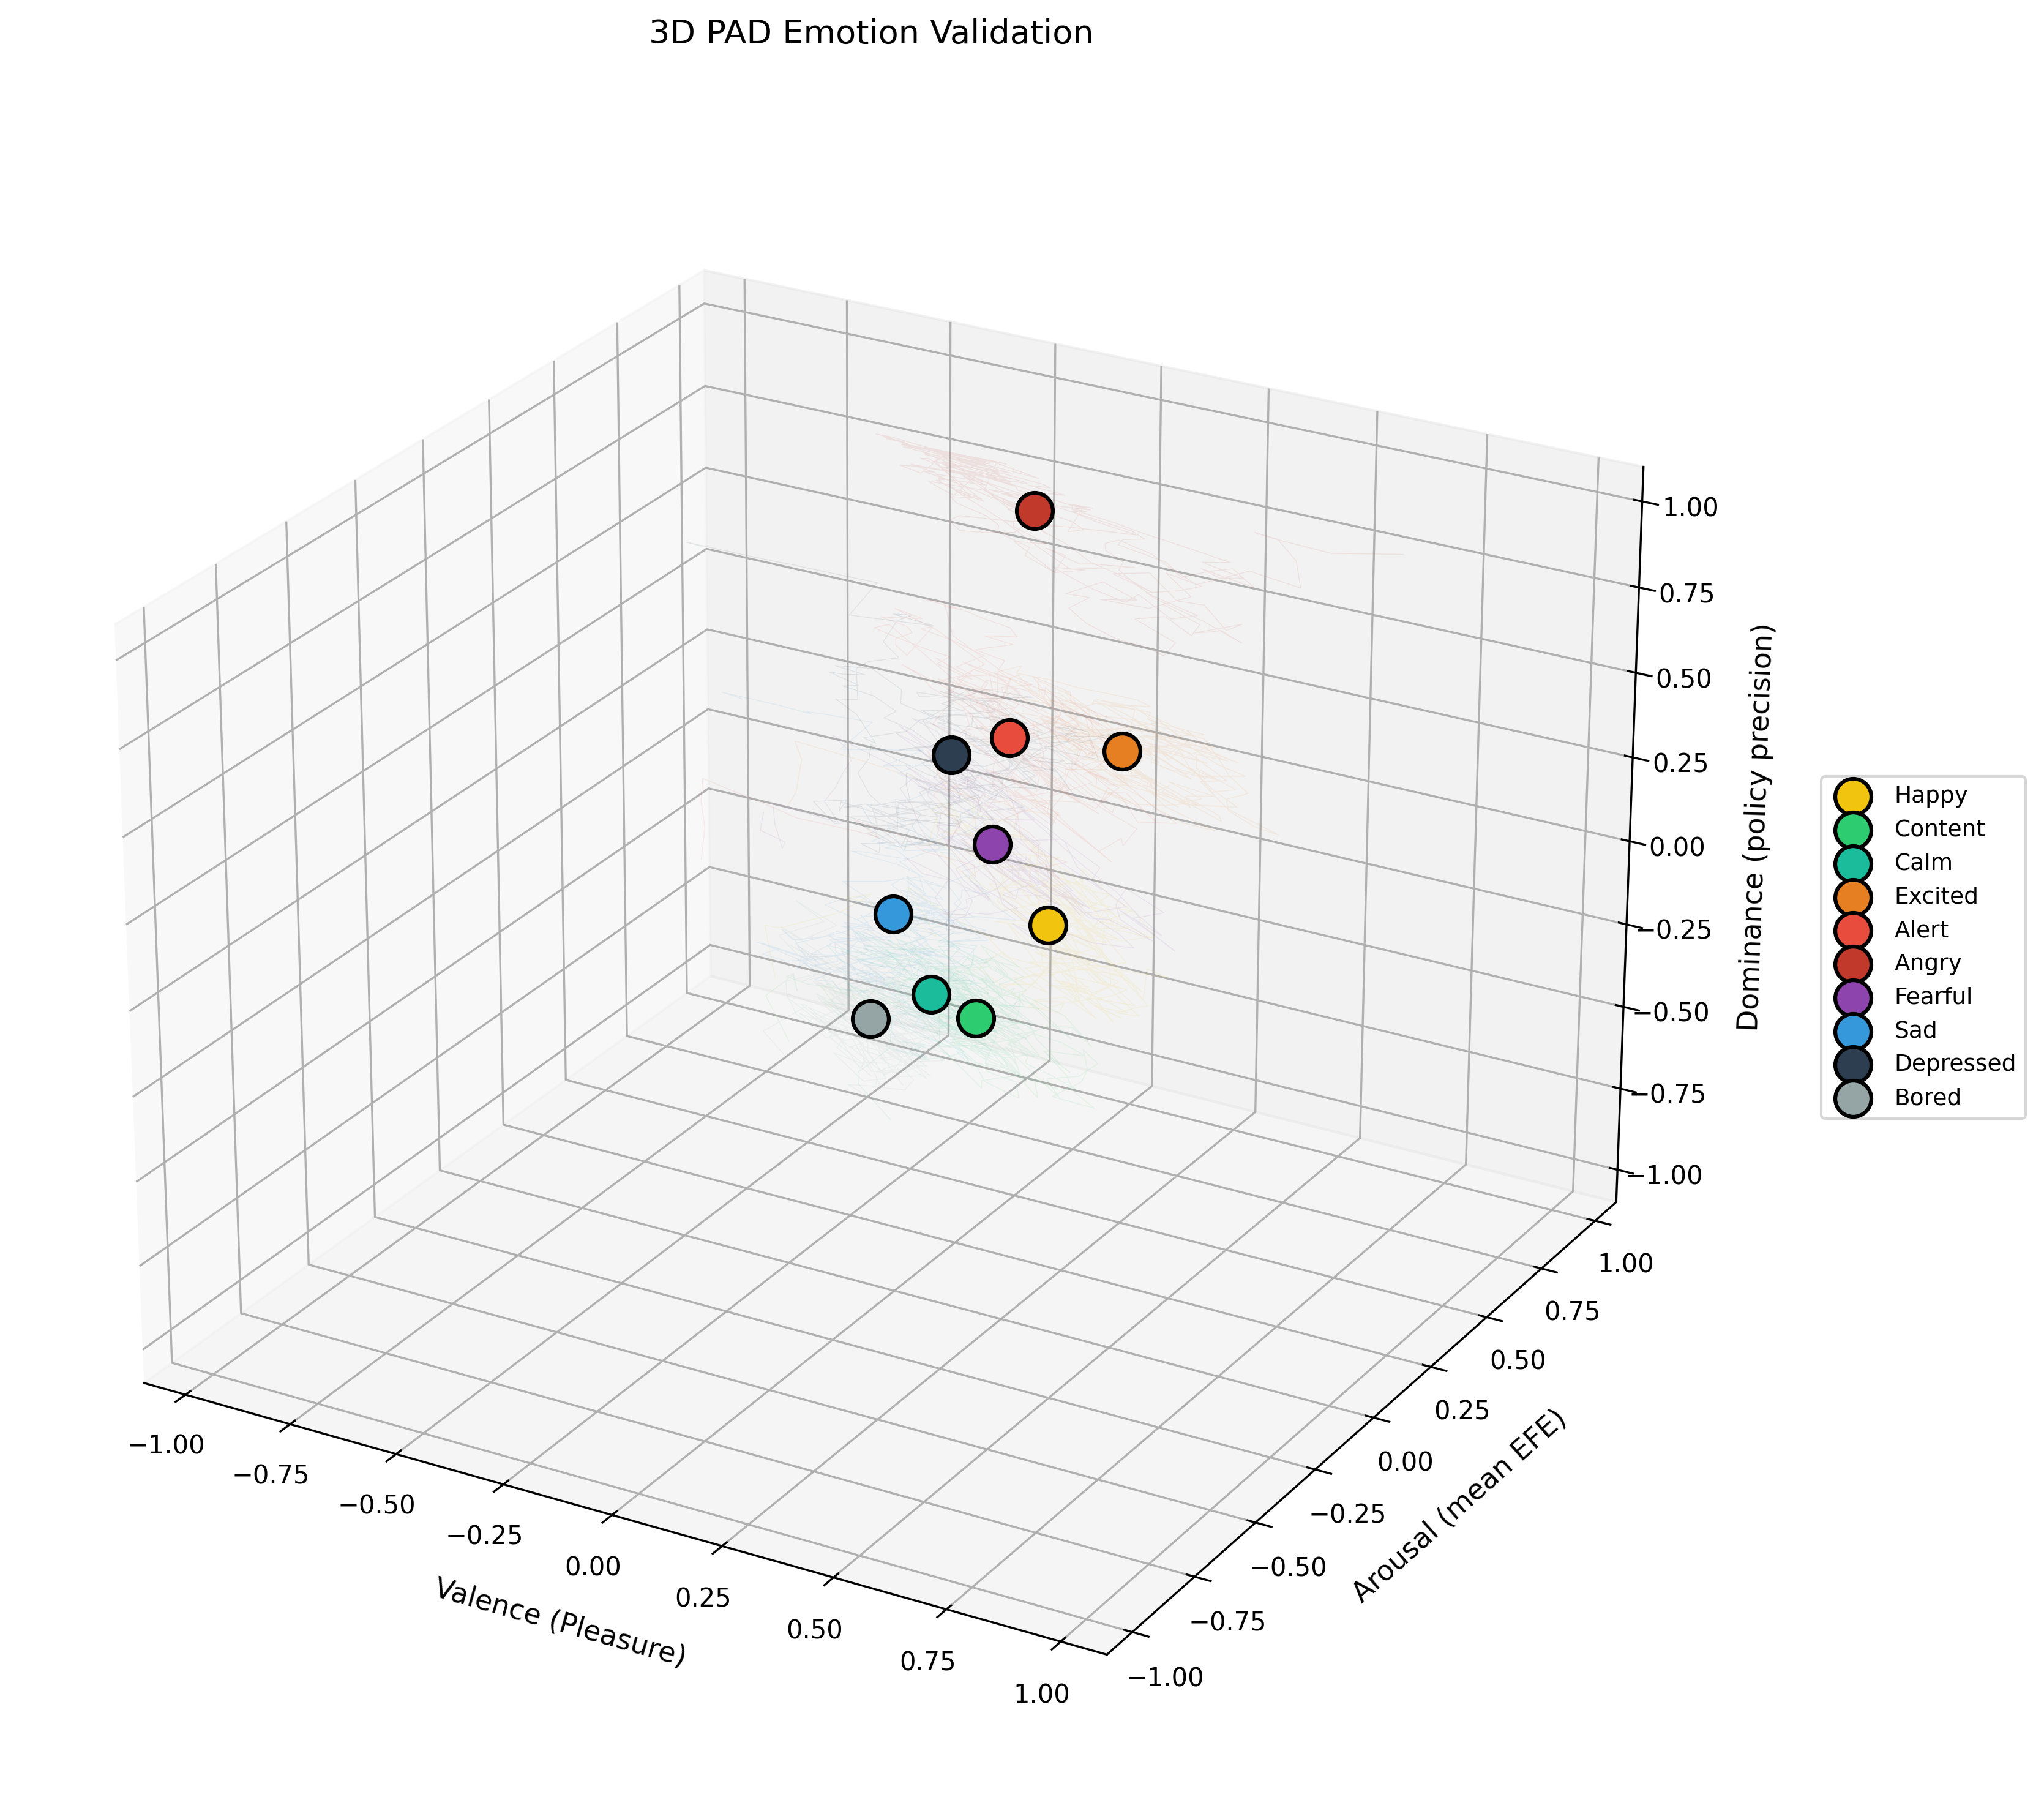
\includegraphics[width=\textwidth]{figures/fig7_emotion_validation.png}
    \caption{\textbf{PAD emotion validation.} Ten emotion profiles embedded in the Pleasure--Arousal--Dominance space. Pleasure is read from composite valence, arousal from mean EFE magnitude, dominance from $1 - H[\pi]/\log|\Pi|$. Profiles cluster in qualitatively correct PAD regions without explicit PAD targeting.}
    \label{fig:emotion_validation}
\end{figure}

\subsection{Limitations and Future Directions}\label{sec:limitations}

Several limitations point toward future work. First, while the M5 mood layer implements a hierarchical POMDP over $\pi_{\text{pos}}$, the emotion-level policy selection remains single-step rather than multi-step planning \citep{friston2018deep}. Extending to deep temporal planning at the emotion level, with multi-step lookahead over temporal frame sequences, would better capture narrative entrenchment and flexibility.

Second, the temporal frame is modelled as a categorical variable ($\{$\textsc{past}, \textsc{present}, \textsc{future}$\}$) rather than a continuous temporal depth. In reality, ``the past'' admits degrees, from last week to childhood, and temporal framing may involve selecting a continuous temporal horizon rather than a discrete category.

Third, the E~vector (habit prior) is currently set as a fixed parameter rather than learned. In reality, ruminative habits develop over time through repeated activation \citep{watkins2008constructive}. A hierarchical model in which the E~vector is itself inferred from accumulated experience, analogous to the M5 mood layer's inference over $\pi_{\text{pos}}$, would capture the \emph{development} of habitual processing styles rather than assuming them as given.

Fourth, the model addresses single-agent temporal framing. Extending to dyadic and multi-agent settings, where agents' temporal frames interact and potentially synchronise, would connect to the geometric hyperscanning framework for affective co-regulation \citep{hinrichs2025temporal} and to the broader project of understanding how shared temporal orientation supports interpersonal coordination \citep{eldar2016mood}.

\bibliographystyle{plainnat}
\bibliography{references}

\end{document}
